% !TeX program = xelatex
% 编译：latexmk -xelatex -interaction=nonstopmode 高等配位化学_复习笔记.tex
\documentclass[UTF8,zihao=5,a4paper,fontset=fandol]{ctexart}
\usepackage[left=23mm,right=21mm,top=23mm,bottom=22mm,headheight=15pt,headsep=7mm]{geometry}
\usepackage{fontspec}
\setmainfont{TeX Gyre Pagella}
\setsansfont{TeX Gyre Heros}
\setmonofont{Latin Modern Mono}[Scale=MatchLowercase]
\usepackage{amsmath,amssymb}
\usepackage{unicode-math}
\setmathfont{TeX Gyre Pagella Math}
\usepackage[version=4]{mhchem}
\usepackage{graphicx,booktabs,tabularx,longtable,array,multicol}
\usepackage{enumitem}
\usepackage[table]{xcolor}
\definecolor{Ink}{HTML}{20384C}
\definecolor{Teal}{HTML}{087F82}
\definecolor{Gold}{HTML}{A16D27}
\definecolor{Muted}{HTML}{5C6C79}
\definecolor{Pale}{HTML}{EEF6F6}
\usepackage{tikz}
\usetikzlibrary{arrows.meta,positioning,calc,decorations.pathreplacing}
\usepackage[most]{tcolorbox}
\usepackage{fancyhdr}
\usepackage{needspace}
\usepackage{hyperref}
\hypersetup{colorlinks=true,linkcolor=Teal,urlcolor=Teal,
  pdftitle={高等配位化学：循序渐进复习笔记},pdfauthor={讲义整理},
  pdfsubject={配位概念、立体化学、分子对称性、群论与光谱应用},bookmarksnumbered=true}
\usepackage{bookmark}
\usepackage{microtype}
\microtypesetup{protrusion=true,expansion=false}
\linespread{1.22}
\setlength{\parindent}{2em}
\setlength{\parskip}{0.25em}
\setlength{\emergencystretch}{1.5em}
\setlength{\tabcolsep}{5pt}
\renewcommand{\arraystretch}{1.25}
\setlist[itemize]{leftmargin=1.7em,itemsep=0.2em,topsep=0.4em,parsep=0pt}
\setlist[enumerate]{leftmargin=1.9em,itemsep=0.25em,topsep=0.4em,parsep=0pt}
\ctexset{
 section={format=\Large\sffamily\bfseries\color{Ink},name={,},number=\arabic{section},
   aftername=\hspace{0.65em},beforeskip=1.5em,afterskip=0.7em},
 subsection={format=\large\sffamily\bfseries\color{Teal},number=\thesection.\arabic{subsection},
   beforeskip=1.1em,afterskip=0.4em},
 subsubsection={format=\normalsize\sffamily\bfseries\color{Ink},beforeskip=0.8em,afterskip=0.3em}}
\setcounter{tocdepth}{1}
\setcounter{secnumdepth}{2}
\pagestyle{fancy}
\fancyhf{}
\fancyhead[L]{\small\sffamily\color{Muted}高等配位化学\quad /\quad 复习笔记}
\fancyhead[R]{\small\sffamily\color{Muted}\nouppercase{\leftmark}}
\fancyfoot[L]{\footnotesize\sffamily\color{Muted}概念\enspace ·\enspace 结构\enspace ·\enspace 对称性\enspace ·\enspace 应用}
\fancyfoot[R]{\small\sffamily\bfseries\color{Teal}\thepage}
\renewcommand{\headrulewidth}{0.3pt}
\renewcommand{\sectionmark}[1]{\markboth{\thesection\quad #1}{}}
\newcommand{\learning}[1]{\par\noindent{\small\sffamily\color{Teal}\textbf{本节目标}\enspace #1}\par}
\newcommand{\sources}[1]{\par\noindent{\footnotesize\color{Muted}讲义定位：#1}\par\vspace{0.35em}}
\newtcolorbox{keyidea}[1][]{enhanced,breakable,colback=Pale,colframe=Teal,
 boxrule=0pt,borderline west={1.2pt}{0pt}{Teal},sharp corners,
 left=9pt,right=9pt,top=7pt,bottom=7pt,before skip=9pt,after skip=9pt,
 title={#1},coltitle=Teal,fonttitle=\sffamily\bfseries,
 attach title to upper={\par\smallskip},colbacktitle=Pale}
\newtcolorbox{worked}[1][]{enhanced,breakable,colback=Gold!4!white,colframe=Gold!45,
 boxrule=0.4pt,arc=1mm,left=9pt,right=9pt,top=7pt,bottom=7pt,
 before skip=9pt,after skip=9pt,title={例题\enspace #1},
 coltitle=Gold,fonttitle=\sffamily\bfseries,attach title to upper={\par\smallskip}}
\newcommand{\partlabel}[2]{\clearpage\markboth{}{}\noindent
 {\small\sffamily\bfseries\color{Teal}#1}\hspace{0.7em}
 {\small\sffamily\color{Muted}#2}\par\vspace{0.25em}}
\begin{document}
\thispagestyle{empty}
\noindent{\small\sffamily\bfseries\color{Teal}课程讲义整理\quad /\quad 第一至三章}
\vspace{1.2cm}

\noindent{\Huge\sffamily\bfseries\color{Ink}高等配位化学}\par
\vspace{0.35cm}
\noindent{\LARGE\sffamily\color{Teal}循序渐进复习笔记}\par
\vspace{0.5cm}
\noindent{\large 从读懂配合物，到用对称性分析结构、光谱与成键。}
\vspace{0.7cm}

\subsection*{先学会这条主线}
\noindent
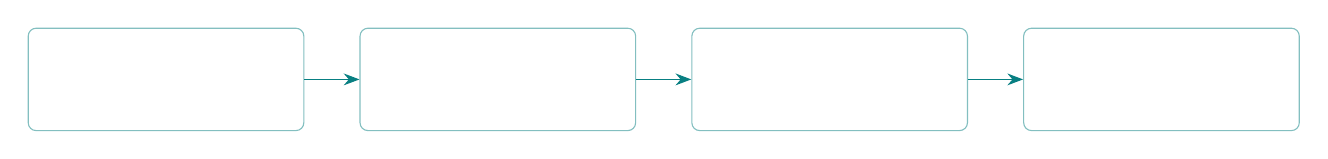
\begin{tikzpicture}[node distance=5mm, every node/.style={font=\small},
 stage/.style={draw=Teal!50,rounded corners=1mm,minimum width=35mm,minimum height=13mm,align=center},
 >={Stealth[length=2mm]}]
\node[stage] (a) {读化学式\\电荷、配位数、配体};
\node[stage,right=7mm of a] (b) {画空间结构\\几何异构、手性};
\node[stage,right=7mm of b] (c) {识别对称性\\点群、表示、约化};
\node[stage,right=7mm of c] (d) {解决具体问题\\振动谱、分子轨道};
\draw[->,Teal] (a)--(b);\draw[->,Teal] (b)--(c);\draw[->,Teal] (c)--(d);
\end{tikzpicture}

\subsection*{怎样使用}
第一遍顺序阅读正文与例题，先把“为什么”和计算步骤接起来。已经熟悉的概念可以略读，但不要跳过点群判定、特征标约化和振动分析的完整算例。

第二遍合上答案完成末尾自测。哪里卡住，就按答案标出的节号回查；最后用一页速查表复述整条解题链。这里的“快速上手”是尽快学会判断与计算，不是只背结论。

\subsection*{四份材料的范围}
\noindent
\begin{tabularx}{\linewidth}{@{}l X r@{}}
\toprule
代号 & 原始讲义 & PDF 页数\\
\midrule
A & 第一章：配位化学发展简史及基本概念 & 79\\
B & 第二章：配合物的立体结构与异构现象 & 70\\
C & 第三章：分子的对称性和群论初步（一） & 44\\
D & 第三章：分子的对称性和群论初步（二） & 57\\
\bottomrule
\end{tabularx}

\vfill
\noindent{\small\color{Muted}正文每节标注讲义定位，页码从各 PDF 的第一页计起。内容覆盖这四份材料；第一章预告的后续课程主题不另行扩写。为便于复算，本文统一符号、补全推导，并将分子异构体与外消旋混合物分开计数。}
\clearpage
\markboth{阅读导航}{阅读导航}
{\small\tableofcontents}
\vspace{0.6em}
\noindent{\small\color{Muted}\textbf{阅读约定}\quad $\Delta/\Lambda$ 表示配位骨架的螺旋构型，$(+)/(−)$ 表示给定条件下的旋光方向；$E$ 既可能指恒等操作，也可能是二维不可约表示的行名，须按上下文区分。}

\partlabel{第一部分\quad 认识配合物}{先读懂化学式，再讨论结构与手性}
\section{读懂配合物}
\learning{能从化学式辨认内外界，分别计算氧化态、配位数与 $d$ 电子数；能把配体的连接方式读出来，并完成简单配合物的双向命名。}
\sources{A，第12--19、26--32、37--46、58--78页；B，第1--3页。}

\subsection{先分清：一个配合物里有哪些结构单元}
配合物由中心原子与配体通过配位作用结合而成。中心通常是金属原子或离子；配体可以是中性分子，也可以是离子。方括号内的\textbf{配位个体}通常称为内界；为平衡电荷而存在、没有直接与该中心配位的离子称为外界。例如，\ce{[Co(NH3)5Cl]Cl2} 的内界是 \ce{[Co(NH3)5Cl]^2+}，外界有两个 \ce{Cl-}。内界本身也可以中性，如 \ce{[Ni(CO)4]}，此时不需要外界反离子。

三个容易混用的计数要分开。\textbf{配位原子}是配体上直接与金属结合的原子；\textbf{齿数}是一个配体实际向同一个金属提供的配位原子数；\textbf{配位数}则是该金属周围直接相连的配位原子总数。乙二胺 en 以两个 N 配位，是双齿配体；\ce{[Co(en)3]^3+} 含三个配体，却是六配位。桥联配体连接多个金属时，要对每个金属分别计数，不能把整个团簇共用的原子只算一次。

螯合配体用两个或更多配位原子结合\emph{同一个}金属，并形成包含金属的环。两可配体则可以换用不同原子配位，如 \ce{NO2-} 的 N 配位与 O 配位；“可以换一个原子”不等于“同时以两个原子螯合”。en 常形成五元螯环；五元、六元环通常较容易适应配位几何，但环大小不是稳定性的唯一判据，还要考虑键角、柔性、金属大小及配体的预组织。

\subsection{氧化态与电子数：先算电荷，再谈成键}
给定配位个体的总电荷 $q$，按约定给配体分配形式电荷 $q_i$，中心金属的氧化态 $x$ 满足
\[
 x+\sum_i q_i=q.
\]
对常见过渡金属，形式 $d$ 电子数可由“族序数减去氧化态”得到。例如，Co 属第9族，Co(III) 为 $d^6$；Ni 属第10族，Ni(II) 为 $d^8$，Ni(0) 为 $d^{10}$。\ce{NH3}、水、en、CO 的形式电荷为0，卤离子为 $-1$，草酸根 ox 为 $-2$。不能因为 CO 能接受反馈电子，就把它按带负电的配体来配平。

氧化态是电子归属的\textbf{记账规则}，不是金属真实电荷的测量值。含配体自由基等非无辜配体的体系，可能存在“金属被氧化”与“配体被氧化”的不同描述；此时需要结合光谱和电子结构证据，不能只靠总电荷认定电子实际在哪里。

\begin{worked}[同一式子，回答四种问题]
求 \ce{[CoCl2(en)2]Cl} 的内外界、Co 氧化态、配位数和 $d$ 电子数。

外界为一个 \ce{Cl-}，所以内界 \ce{[CoCl2(en)2]+} 带 $+1$ 电荷。由 $x+2(-1)+2(0)=+1$ 得 Co 为 $+3$ 价。两个 en 各提供两个 N，两个氯各提供一个 Cl，因此配位数是 $2\times2+2=6$，而配体数是4。Co(III) 的形式电子组态为 $d^6$。式子尚未写出 cis 或 trans，因而\emph{没有唯一指定几何异构体}。
\end{worked}

\subsection{常见配体：记住电荷、给体原子与连接限制}
下表将常见的形式电荷、给体原子和连接约束放在一起；实际齿数仍由具体结构确定。

\begin{center}
\small
\begin{tabularx}{\linewidth}{@{}l c l X@{}}
\toprule
配体或缩写 & 电荷 & 常见给体／齿数 & 做题时要留意的事 \\
\midrule
\ce{NH3}、\ce{H2O} & 0 & N、O；单齿 & 氨与水均不带电 \\
\ce{Cl-}、\ce{Br-} & $-1$ & 卤素；单齿 & 可端基配位，也可桥联 \\
\ce{CN-} & $-1$ & 常为 C；单齿 & 也可经 N 配位或桥联 \\
\ce{NO2-} & $-1$ & N 或 O；常为单齿 & 需标明是 N 配位还是 O 配位 \\
\ce{SCN-} & $-1$ & S 或 N；常为单齿 & SCN 与 NCS 的写法提示连接端 \\
CO & 0 & C；单齿 & $\sigma$ 给电子、$\pi$ 接受电子 \\
en & 0 & N,N；双齿 & 乙二胺，柔性五元螯环 \\
bpy、phen & 0 & N,N；双齿 & 2,2$'$-联吡啶、1,10-菲咯啉，骨架较刚性 \\
ox、acac & $-2$、$-1$ & O,O；双齿 & 分别为草酸根、乙酰丙酮根 \\
terpy & 0 & N,N,N；三齿 & 三联吡啶，通常要求近似 mer 的排列 \\
trien、tren & 0 & 四个 N；四齿 & 线性链与支化骨架，几何约束不同 \\
edta & $-4$ & 常为 N$_2$O$_4$；六齿 & 必须区分 edta$^{4-}$ 与其质子化形式 \\
\bottomrule
\end{tabularx}
\end{center}

\subsection{配位键不只是“画一个箭头”}
用 $L\to M$ 表示配体向金属提供电子对，强调的是成键轨道的来源。成键以后，电子处在整个配合物的分子轨道中；配位键并不是一种永远只能由一方“拥有电子”的特殊共价键。实际金属--配体键通常同时具有共价性和静电作用，也不能仅凭某个固定的电负性差阈值把所有键二分。

氨可用 N 上的孤对电子向金属提供 $\sigma$ 相互作用。CO 则既以 C 端孤对电子给电子，又用空的 $\pi^*$ 轨道接受金属 $d_\pi$ 电子，形成\textbf{$\pi$ 反馈}。两种作用常相互协同；反馈会占据配体的反键轨道，使 C--O 键趋于减弱。烯烃配位也是类似的授受组合：烯烃的已占据 $\pi$ 轨道向金属给电子，金属向烯烃空的 $\pi^*$ 轨道反馈。蔡司盐中的乙烯正是这一模型的代表。这里“$\sigma$ 给电子”描述相对于金属--烯烃连接方向的对称性，并不意味着电子必须来自烯烃的 $\sigma$ 键。

卤离子等配体还可通过已占据的 $\pi$ 轨道向金属给电子，属于 $\pi$ 给体；CO 等接受金属反馈电子的配体则属于 $\pi$ 受体。比较配体时，应分别说明 $\sigma$ 与 $\pi$ 相互作用中的电子流向。

\textbf{配位层}帮助我们从局部结构逐层看向整个配体。第一层关注金属与直接配位原子；第二层关注把这些原子连接起来的螯合骨架；更外层包括取代基等部分，它们可以改变位阻、诱导效应及分子间作用。\ce{[Co(NH3)6]^3+} 与 \ce{[Co(en)3]^3+} 都有 CoN$_6$ 第一层，但后者的 N 被成对连起来，能形成有手性的螺旋排列。这种结构差异要到第二层才看得出来。

\subsection{Werner 的证据链：从组成走向空间结构}
Werner 在1893年提出配位理论，把当时的主价、副价分别与今日的氧化态、配位数相联系，并强调配位有确定的空间方向。其说服力不只来自某一种颜色或某一次分析，而来自组成、反应、溶液性质与异构体数目之间的相互制约。

\begin{center}
\small
\begin{tabularx}{\linewidth}{@{}l c c X@{}}
\toprule
化合物 & 迅速沉淀的 Cl$^-$ & 理想离子数 & 结构解释 \\
\midrule
\ce{[Co(NH3)6]Cl3} & 3 & 4 & 三个氯均在外界 \\
\ce{[CoCl(NH3)5]Cl2} & 2 & 3 & 一个氯进入内界，仍为六配位 \\
\ce{[CoCl2(NH3)4]Cl} & 1 & 2 & 两个氯在内界，可出现 cis/trans \\
\ce{[CoCl3(NH3)3]} & 0 & 0 & 中性内界，可出现 fac/mer \\
\bottomrule
\end{tabularx}
\end{center}

表中的沉淀量指每摩尔化合物在适当条件下与 \ce{Ag+} 快速反应所得 \ce{AgCl} 的摩尔数；离子数按内界保持完整、理想电离计算。电导率与依数性支持不同的外界离子数，但电导率并不与离子数严格成比例。六配位系列的几何异构体数进一步支持八面体，而不是只凭“六配位”就宣布必为八面体。1911年对手性钴配合物的成功拆分，又证明配体确实具有可分辨的三维排列；后来不含碳的配合物也被拆分，说明手性不以不对称碳为必要条件。

\subsection{从式到名，再从名还原化学式}
命名可分成两层：先说清\emph{一个配位个体}中的配体、数目、连接方式和金属氧化态，再按盐的组成连接内外界名称。本笔记沿用讲义的中文配体排列习惯：无机配体在有机配体之前，同类中通常先阴离子后中性配体，再依据给体原子等规则排列。不要把这套中文顺序与英文系统命名的字母排序拼接使用。复杂配体的数目用括号隔开，例如“三(乙二胺)”，避免把配体名称中的数字误读为个数。

简单外界阴离子常用“氯化……”这样的盐名，含氧酸根用“硫酸……”“硝酸……”；配阴离子的盐通常写作“……合某金属酸某”。例如 \ce{K2[PtCl6]} 为六氯合铂(IV)酸钾，\ce{[Co(NH3)6]Cl3} 为氯化六氨合钴(III)。几何信息用 cis、trans、fac、mer 放在名称或配位个体之前，不能指望只写组成就能还原空间排列。

连接标记中，\textbf{$\kappa$ 指出具体的配位原子}，如亚硝酸根-$\kappa N$ 与亚硝酸根-$\kappa O$；en 的 $\kappa^2N,N'$ 表示两个 N 都与同一中心结合。\textbf{$\eta$ 表示同一连续片段参与配位的原子数}，如二茂铁 \ce{[Fe(C5H5)2]} 中每个茂环为 $\eta^5$，乙烯常为 $\eta^2$。它不是两个孤立给体原子的齿数记号。讨论 $\pi$ 配体的“配位数”时应先声明按原子还是按配位位点计数；不能把传统的空间位点数与逐原子计数混加。

\textbf{$\mu$ 表示桥联}，$\mu_2$ 表示连接两个中心，通常可简写为 $\mu$。例如 \ce{[(NH3)5Cr(OH)Cr(NH3)5]Cl5} 可称五氯化($\mu$-羟)·二[五氨合铬(III)]；一个桥联 \ce{OH-} 同时为两个 Cr 各贡献一个 O 配位原子。名称中的“羟”不应被误读为中性水。

\begin{worked}[把名字中的信息逐项还原]
“氯化氯·五氨合钴(III)”对应什么式子？“反-四(异硫氰酸根)·二氨合铬(III)酸铵”又怎样还原？

第一例的内界含 Co(III)、一个 \ce{Cl-} 和五个中性氨，净电荷为 $+2$，需两个外界氯离子，故为 \ce{[CoCl(NH3)5]Cl2}。开头的“氯化”与内界名称中的“氯”不是重复计数。

第二例内界电荷为 $+3-4=-1$，故为 trans-\ce{NH4[Cr(NCS)4(NH3)2]}。“异硫氰酸根”在此表示经 N 配位，也可用 $\kappa N$ 明示；trans 指两个氨互处反位。检验时同时检查总电荷为零、配位数为6和 N 配位方式，三项都满足才算还原完整。
\end{worked}

\section{从配位数到空间构型}
\learning{知道常见配位数对应哪些候选构型，能解释四配位和六配位的主要选择，并把金属电子结构、配体约束与结构互变联系起来。}
\sources{B，第1--9、27--32页；A，第73--78页。}

\subsection{配位数给候选，不给唯一答案}
确定空间构型时，先数金属周围的实际配位原子，再比较候选多面体。下面的名称说的是\emph{配位原子的位置}，不是整个配合物的外形；实际结构允许有键长、键角和扭转的偏离。

\begin{center}
\small
\begin{tabularx}{\linewidth}{@{}c l X@{}}
\toprule
配位数 & 主要候选构型 & 如何识别或理解 \\
\midrule
2 & 直线形 & 两个方向近似相反，Au(I)、Ag(I) 常见 \\
3 & 平面三角形；三角锥 & 前者金属与三个给体近共面，不是四面体少画一键 \\
4 & 四面体；平面四方形 & 是否共面、是否有 $180^\circ$ 反位关系是关键 \\
5 & 三角双锥；四方锥 & 分别为三赤道加两轴向、四基面加一顶点 \\
6 & 八面体；三棱柱 & 前者有三对反位，后者有两个近重叠的平行三角面 \\
7 & 五角双锥；单帽八面体；单帽三棱柱 & “加帽”是在原多面体某一面的外侧增加顶点 \\
8 & 四方反棱柱；三角十二面体等 & 也可见立方体、双帽三棱柱、六角双锥 \\
\bottomrule
\end{tabularx}
\end{center}

\subsection{四配位：为什么 $d^8$ 不是充分条件}
四面体的四个配位方向彼此等价，没有一对配体严格处于反位；平面四方形则有两对相对位置，因而能支持常见的顺反异构。几何选择要比较电子能量与配体间排斥，不能仅凭配位数区分，也不能把杂化轨道标签当成结构选择的独立原因。

对 $d^8$ 金属，平面四方形分裂常把一个强反键的 $d$ 轨道抬得很高，使八个电子占据其余轨道而获得有利排布。Pd(II)、Pt(II) 的四配位配合物通常倾向平面四方形；Ni(II) 则对配体及环境更敏感。典型地，\ce{[Ni(CN)4]^2-} 为平面四方形、抗磁，\ce{[NiCl4]^2-} 为四面体、顺磁：二者都是 Ni(II)、$d^8$，电子数并没有改变。

在一些 Ni(II) 配合物中，平面形与四面体形的能量差不大，改变配体、溶剂或温度便可能改变平衡。讲义中的膦配合物体现了这种构型与磁性的联系。磁性可以作为构型线索，再与组成、光谱及衍射证据相互印证。

\subsection{五配位互变、六配位的两个三角面}
三角双锥中，轴向配体与三个赤道配体分别约成 $90^\circ$，赤道配体之间约成 $120^\circ$；四方锥则有四个近共面的基面位置与一个顶端位置。真实五配位结构常位于两者之间。\textbf{Berry 假旋转}使两个轴向位置与两个赤道位置交换，途经近似四方锥的几何，另一个赤道位置在这次过程中不参与交换。它不需要先把配体完全解离；若互变比谱学观测快，原本不等价的位置可能表现为时间平均等价。

六配位以八面体最常见，但不是只有八面体。可把八面体看作两个相对的三角面，沿共同轴投影时呈交错排列；三棱柱的两个三角面近似重叠。两者之间的扭转提供了理解构型变形的直观路径。讲义中的三(二硫烯)铼配合物 \ce{[Re(S2C2(CF3)2)3]} 是三棱柱结构的例子。某些金属与受限的螯合骨架会稳定这种排列，所以看到六个配位原子时，仍要检验反位关系和三角面的相对取向。

\subsection{七、八配位：用“底面、扭转、加帽”读图}
七配位可以从一个五边形加上下两个顶点得到五角双锥；也可以从六配位多面体出发，在一个面外加帽。同样是七配位，晶格与反离子环境也可能改变哪一种结构更稳定。配位数相同，不保证两个晶体拥有同一多面体。

八配位的\textbf{四方反棱柱}可由立方体帮助想象：保留上下两个正方形，把其中一个绕中心轴转动约 $45^\circ$，上下顶点便交错排列；连接相邻顶点后，侧面由四边形变成三角形。\textbf{三角十二面体}有八个顶点、十二个三角面，名称中的“十二”指面数，不是配位数。可把立方体的顶点交替分成两组四面体，再对两组作不同的拉伸、压缩来理解其变形。它也不是有二十个顶点的正十二面体。双帽三棱柱是在三棱柱基础上再加两个帽；六角双锥则是六个赤道点加两个轴向点。

\subsection{结构选择时按什么顺序分析}
先看\textbf{金属容纳空间}：较大的金属与较小的给体往往较容易形成高配位数；氧化态升高可加强吸引，却也会改变金属半径，不能只记“电荷越高，配位数越大”。稀土和较大的早过渡金属常见高配位数。$d^0$ 体系没有传统的 $d$ 电子配体场稳定化能，不能把它们的高配位直接归因于“得到更多配体场稳定化能”。

再看\textbf{配体是否装得下、够不够得着}：体积大的配体会增加排斥，多齿配体的齿间距离和咬合角则限制可占据的位置。最后比较\textbf{电子结构与环境}：$d$ 电子数、$\sigma/\pi$ 成键、溶剂配位、反离子及晶体堆积都会参与选择。

\section{枚举异构体与判断手性}
\learning{先按连接关系分类，再按几何关系与镜像关系计数；会用明确坐标枚举八面体异构体，并把单分子立体异构体与样品混合物分开。}
\sources{B，第10--25、29--48、61--65页；A，第37--44、67--78页。}

\subsection{第一道分岔：连接关系变了没有}
同分异构体具有相同的总组成，却不是同一个结构。先问金属与哪些原子相连、哪些物种在内界；若这些连接不同，属于结构异构。若连接相同而空间排列不同，才进入立体异构的讨论。

\begin{center}
\small
\begin{tabularx}{\linewidth}{@{}l X X@{}}
\toprule
类型 & 一组典型例子 & 实际改变了什么 \\
\midrule
配位异构 & \ce{[Co(NH3)6][Cr(ox)3]} 与 \ce{[Cr(NH3)6][Co(ox)3]} & 配阳、配阴离子之间交换了配体的归属 \\
键合异构 & \ce{[Co(NO2)(NH3)5]^2+} 与 \ce{[Co(ONO)(NH3)5]^2+} & 同一个两可配体换用 N 或 O 配位 \\
电离异构 & \ce{[CoBr(NH3)5]SO4} 与 \ce{[Co(SO4)(NH3)5]Br} & 内外界交换，直接释放的外界离子不同 \\
水合异构 & \ce{[Cr(H2O)6]Cl3} 与 \ce{[CrCl(H2O)5]Cl2.H2O} & 水在配位水与结晶水之间改变归属 \\
\bottomrule
\end{tabularx}
\end{center}

水合异构属于溶剂合异构的特例。比较时应把结晶水计入总组成，不能因为它在方括号外就忽略。配体自身若换成另一种连接异构体，例如1,2-丙二胺换成1,3-丙二胺，相应配合物也改变了结构；这与同一配体换配位原子的键合异构不是同一层次。

\subsection{把 cis/trans 和 fac/mer 放在明确的位置上}
平面四方形中，cis 表示指定的两个配体相邻，夹角约 $90^\circ$；trans 表示相对，约 $180^\circ$。四面体中任意两个顶点的关系相同，不能照搬平面形的 cis/trans。下面两图只画金属与配位原子的连接，不表示键长比例。

\begin{center}
\begin{tikzpicture}[every node/.style={font=\small},line width=.6pt]
\begin{scope}[xshift=-2.6cm]
\node (m) at (0,0) {Pt};
\node (t) at (0,1) {Cl}; \node (r) at (1.3,0) {Cl};
\node (b) at (0,-1) {$\mathrm{NH_3}$}; \node (l) at (-1.3,0) {$\mathrm{H_3N}$};
\draw (m)--(t) (m)--(r) (m)--(b) (m)--(l);
\node at (0,-1.65) {cis：两个 Cl 相邻};
\end{scope}
\begin{scope}[xshift=2.6cm]
\node (m) at (0,0) {Pt};
\node (t) at (0,1) {Cl}; \node (r) at (1.3,0) {$\mathrm{NH_3}$};
\node (b) at (0,-1) {Cl}; \node (l) at (-1.3,0) {$\mathrm{H_3N}$};
\draw (m)--(t) (m)--(r) (m)--(b) (m)--(l);
\node at (0,-1.65) {trans：两个 Cl 相对};
\end{scope}
\end{tikzpicture}
\end{center}

八面体可统一用六个位置 $+x,-x,+y,-y,+z,-z$ 表示：同一轴的正负端互为 trans，不同轴的任意两端互为 cis。对 $MA_3B_3$，三个 A 占据一个三角面时为 fac；三个 A 中有一对反位、三者与金属共处一个经面时为 mer。下面的占位表可直接用来画模型，未列出的配体填满其余位置。

\begin{center}
\small
\begin{tabular}{@{}lll@{}}
\toprule
组成与形式 & 指定配体的占位 & 一眼检查的条件 \\
\midrule
$MA_4B_2$，trans & B 在 $+z,-z$ & 两个 B 相对 \\
$MA_4B_2$，cis & B 在 $+z,+x$ & 两个 B 相邻 \\
$MA_3B_3$，fac & A 在 $+x,+y,+z$ & A 之间三组关系全为 cis \\
$MA_3B_3$，mer & A 在 $+x,-x,+z$ & A 中恰有一组 trans \\
\bottomrule
\end{tabular}
\end{center}

\subsection{计数先固定模型，再消去重复}
枚举时先说明配体是否单齿、双齿是否对称，是否忽略螯环构象与配位 N 的手性。随后固定一个配体位置，依据剩余位置的相邻、相对关系分类，并用\emph{整体旋转}消去重复。镜面反射不能用于把两个对映体合并；只有在专门统计“几何类型”时，才把一对对映体归入同一类。

下表把几何类型与分子立体异构体数并列。A、B 等为不同的无手性单齿配体，AA 为对称双齿配体；忽略环构象和配体自身手性。“几何类型”一栏按不分镜像的一对计一个类型。

\begin{center}
\small
\begin{tabularx}{\linewidth}{@{}l c c X@{}}
\toprule
模型 & 几何类型 & 立体异构体 & 计数原因 \\
\midrule
平面 $MA_2B_2$ & 2 & 2 & cis、trans，均无手性 \\
平面 $MABCD$ & 3 & 3 & 固定 A，再选其反位配体，有三种选择 \\
四面体 $MABCD$ & 1 & 2 & 一对不能重合的镜像 \\
八面体 $MA_4B_2$ & 2 & 2 & cis、trans，均无手性 \\
八面体 $MA_3B_3$ & 2 & 2 & fac、mer，均无手性 \\
八面体 $MA_2B_2C_2$ & 5 & 6 & 全反1种、恰一对反位3种、全顺1对对映体 \\
八面体 $M(AA)_3$ & 1 & 2 & $\Delta$、$\Lambda$ 一对 \\
八面体 $M(AA)_2B_2$ & 2 & 3 & trans 1个；cis 为一对对映体 \\
八面体 $MABCDEF$ & 15 & 30 & 六种配体全不同，15对对映体 \\
\bottomrule
\end{tabularx}
\end{center}

对最后一行，可以先把六个配体分为三组反位配对，共有 $5\times3\times1=15$ 种。每个配对方案仍有两个相反的空间手性；不同配体全部标记后，不存在能把两者重合的镜面或反心。因此分子总数是30，不是15。这个思路比画30个没有位置标记的八面体更容易查错。

\subsection{镜像、手性与构象：三个问题不要互相代替}
\textbf{对映体}互为镜像而不能经整体旋转重合；\textbf{非对映异构体}是彼此不呈镜像关系的立体异构体，例如 cis 与 trans。非对映异构体不要求双方都有手性。判断一个指定结构是否有手性，应检查它能否与镜像重合；等价的对称性判据是不存在任何反轴 $S_n$，其中也包括镜面 $S_1$ 和反心 $S_2$。只有“没有反心”远远不够，含镜面的结构仍然无手性。

无手性配体也能排出有手性的整体。\ce{[Co(en)3]^3+} 的三个螯环像螺旋桨，形成右手 $\Delta$ 与左手 $\Lambda$ 两种构型。判读时沿选定的三重轴看螯合带向远处延伸的旋向，并与右手或左手螺旋比较；先标明观察方向，不能只凭纸面上线条的斜率猜。大写 $\Delta/\Lambda$ 描述整体螯合排列，小写 $\delta/\lambda$ 可描述五元螯环的局部构象，二者不是同一个标签。对于 edta 等多齿配体，还需要按明确的螯环组合规则指定，不能随意套用三条等价螯合带的图像。

\textbf{构象异构}来自单键转动或环翻转等变化，通常不改变原子连接，也不一定改变金属中心构型。例如 en 环的翻转可以改变环褶皱而不改变整个三螯合体的 $\Delta/\Lambda$。若转动能垒很高，阻转异构体可在实验时间尺度上分离；若互变很快，谱学看到的可能只是平均结构。是否能分离，必须连同温度与观测时间说明。

\begin{keyidea}[构型符号不是旋光方向]
$\Delta/\Lambda$、$R/S$ 是空间构型标签；$(+)/(−)$ 是在指定波长、溶剂、温度等条件下测得的旋光符号，二者没有普遍的一一对应关系。同一构型在不同波长下甚至可能改变旋光符号。外消旋样品含等量对映体，净旋光可相消，但其中的每一个分子仍可有手性。$rac$ 是样品组成说明，不是新增的分子异构体。
\end{keyidea}

\subsection{trien 与 tren：同为四齿，限制却不同}
trien 是线性的三乙四胺，四个 N 按 $N_1$--$N_2$--$N_3$--$N_4$ 连成一条链；tren 是三(2-氨乙基)胺，一个中心 N 连着三条含端基 N 的支臂。二者都能提供四个 N，但不能任意交换它们在八面体上的位置。下面采用讲义的常见五元螯环模型，不计配位 N 的独立手性，也不把不同环褶皱拆成新异构体。

\begin{worked}[{用坐标完整枚举 $[MX_2(\mathrm{trien})]$ 与 $[MX_2(\mathrm{tren})]$}]
以 $\pm x,\pm y,\pm z$ 为八面体六个顶点，X 是两个相同的单齿配体。trien 的相邻 N 必须占据相邻顶点，以便形成三个常见五元螯环。以下每行给出一份可重建的代表结构；连线顺序严格是 $N_1\to N_2\to N_3\to N_4$，而不是任意把四个 N 两两相连。

\begin{center}
\footnotesize
\begin{tabular}{@{}llll@{}}
\toprule
形式 & 两个 X 的位置 & trien 四个 N 的链路径 & 理想点群 \\
\midrule
trans & $+z,-z$ & $+x\to+y\to-x\to-y$ & $C_{2v}$ \\
cis-a & $+x,+z$ & $+y\to-x\to-z\to-y$ & $C_2$ \\
cis-b & $+x,+z$ & $+y\to-x\to-y\to-z$ & $C_1$ \\
\bottomrule
\end{tabular}
\end{center}

cis-a 的两个末端 N 互处反位，cis-b 的两个末端 N 互为顺位，因此两者不能靠整体旋转变成同一种连接排列。trans 含镜面，无手性；两种 cis 均有手性。将坐标作镜像变换 $(x,y,z)\mapsto(x,-y,z)$，即可分别得到 cis-a 与 cis-b 的另一对映体。故 trien 有 \textbf{3种几何类型，5个分子立体异构体}：$1+2+2$。

对 tren，中心 N 必须与三个支臂末端 N 分别形成螯环。可取中心 N 在 $+z$，三个末端 N 在 $+x,-x,+y$，剩余两个 X 在 $-y,-z$，互为 cis。三个相同支臂的置换不会产生新的几何类型；在此模型下理想点群为 $C_s$，有镜面，故只有\textbf{1种几何类型、1个无手性分子立体异构体}。若进一步计入柔性环的冻结构象，可能出现额外的构象手性，但那是另一层计数。

\end{worked}

\subsection{如何用实验证据区分异构体}
衍射给出连接与空间排列；溶液 NMR 比较等价环境及其相互关系，快速交换时需采用时间平均结构解释。偶极矩利用键偶极的矢量相消区分某些顺反异构体；IR 则比较目标振动的对称性与谱带数，具体计算见第9节。电子光谱提供能级与跃迁强度的信息，可与上述证据配合使用。成功拆分能证明存在可分离的对映体，拆分失败则不足以判断有无手性。

\section{手性表征与不对称催化}
\learning{分清分子手性、晶体手性与样品对映组成，知道绝对构型的证据来源；会计算 ee 与 dr，并能解释普通动力学拆分的转化率限制。}
\sources{B，第33--39、49--60、66--70页；A，第38--45、52页。}

\subsection{外消旋样品结晶后，有三种不同的固态组织}
设一对对映体为 R 与 S。总量各半只规定总体组成，不规定它们怎样进入晶体。

\begin{center}
\small
\begin{tabularx}{\linewidth}{@{}l X X@{}}
\toprule
固态形式 & 单颗晶体内部 & 对分离的含义 \\
\midrule
外消旋混合物（聚集体） & 理想情况下，R 晶体与 S 晶体各自形成 & 可有自发拆分；整个晶体批次仍可为1:1 \\
外消旋化合物 & R、S 在同一晶格中按确定比例有序排列 & 不能靠挑出两类对映纯晶体直接拆分 \\
外消旋固体溶液（假外消旋体） & R、S 可统计性占据晶格位置，组成可变 & 不能仅凭单颗晶体就假定其对映纯 \\
\bottomrule
\end{tabularx}
\end{center}

自发拆分说的是对映体在结晶时分别成晶，并不自动等于整批产物获得非零 ee。若两类晶体恰好等量，混合溶解后仍不旋光。机械挑晶、优先结晶等方法的适用性依赖固相性质；另一种常见拆分思路是加入对映纯拆分剂，把一对对映体转成性质不同的非对映盐或配合物，分离后再除去拆分剂。Werner 钴配合物的经典拆分就利用了这种差别。

还要区别\textbf{分子手性与晶体手性}。无手性的分子或离子也可能按手性方式堆积；讲义中的氯酸钠晶体就是代表。晶体溶解后若手性仅来自堆积，堆积被破坏，溶液不必保留旋光。反之，对映纯且构型稳定的手性配合物溶解后仍可保持分子手性。只含平移、旋转、螺旋操作的 Sohncke 空间群允许手性晶体，但空间群名称本身不能证明分子对映纯，更不能替代绝对构型测定。

\subsection{绝对构型的三类证据，以及 HPLC 能回答什么}
\textbf{反常 X 射线衍射}利用反常散射造成的衍射强度差别区分相反的绝对结构，是直接测定的重要方法。可靠判定需要足够的反常信号、合适的数据与结构模型，并通过绝对结构参数等指标评估；元素、波长、晶体质量和孪晶情况都会影响结果。

\textbf{电子圆二色 ECD／旋光色散 ORD}可通过已知参照物的 Cotton 效应或理论计算间接关联构型。参照物应有相近的空间结构、电子结构与跃迁归属。\textbf{振动圆二色 VCD}比较左、右圆偏振红外吸收差，常结合构象搜索和计算谱，判定哪一绝对构型更符合实验。这两类方法都需要把样品的主要构象与溶剂条件纳入比较。

\textbf{手性 HPLC}用于分离对映体并测定比例；绝对构型则需要通过已知标准品、可靠关联或联用证据指认，不能只根据先后出峰命名。测定比例时应保证分离充分，并确认检测响应。

\subsection{ee 与 dr：先说明分母里有哪些物种}
一对对映体的对映体过量定义为
\[
 ee=\frac{|n_R-n_S|}{n_R+n_S}\times100\%.
\]
报告时应同时指出哪一个占优；也可用带符号形式表达方向，但要说明约定。若 R、S 是唯一两种组分，则主对映体与次对映体的摩尔分数分别为 $(1+ee)/2$ 和 $(1-ee)/2$，此处 ee 代入小数形式。ee 不是主对映体含量，也不是产率。

非对映比 dr 比较指定非对映异构体的量，例如 syn:anti 或某两个相对构型家族。一个分子不一定要有两个不对称碳才有非对映异构体；顺反关系、金属构型与配体手性的组合都可能产生非对映关系。若每一非对映家族内部又有一对对映体，dr 与 ee 必须分别报告，不能相互替代。

\begin{worked}[同一组数据，同时求 dr 与各自的 ee]
样品含两组非对映异构体：A 家族的两个对映体为72和8份，B 家族为12和8份；各数字是已经校正响应的相对摩尔量，总量为100份。
\[
 \mathrm{dr}(A:B)=(72+8):(12+8)=80:20=4:1.
\]
A 家族的 $ee_A=(72-8)/80=80\%$，B 家族的 $ee_B=(12-8)/20=20\%$，各以前一个对映体占优。不能把72除以100叫作72\% ee，也不能把四个组分硬合并成一个没有定义的“总 ee”。若只有一对对映体且 $ee=90\%$，其组成才是95:5，而不是90:10。
\end{worked}

\subsection{手性催化怎样让两条反应路径不再等价}
前手性底物在无手性环境中从两个对映面反应，常形成一对对映产物；引入手性金属--配体环境后，两条路径的过渡态成为非对映关系，能垒便可以不同。底物先配位，配体的空间限制、电子作用和定向相互作用共同影响其取向及成键路径。因此，不对称催化并不只是“用大基团挡住一面”，更准确的任务是比较通向两个产物的完整过渡态。

若两条不可逆平行路径分别给出 R、S，且产物生成后不再消旋，速率差可表现为产物比。高 ee 表示选择性高，却不保证转化率、产率或催化剂稳定性高。讲义中的手性铑膦催化不对称氢化说明，金属提供反应活性，手性配体使反应路径不等价；后续结晶还可能进一步富集优势对映体。这些步骤的贡献应分开描述。

\subsection{普通动力学拆分为什么有50\%的单一对映体上限}
不对称催化通常把前手性底物转成手性产物；\textbf{普通动力学拆分}则从外消旋底物出发，使一个对映体反应得快、另一个慢，从而同时富集产物与未反应底物。它并不是“只有一个对映体能反应”的同义词；那只是选择性无限大时的理想极限。动力学拆分也可以使用手性催化剂，所以二者的差别在底物与选择方式，不在于有没有催化剂。

\begin{worked}[转化率超过一半后，纯度为何下降]
从100 mmol 外消旋底物出发，R、S 各50 mmol。设 R 先完全反应，反应保持立体信息且产物不消旋。在50\%转化率时，可得50 mmol 对映纯的 R 来源产物，并留下50 mmol 对映纯 S 底物。

若继续反应至60\%转化率，就必须再消耗10 mmol S。产物现含50 mmol R 来源产物和10 mmol S 来源对映产物，因此
\[
 ee_P=\frac{50-10}{60}\times100\%=66.7\%.
\]
一般地，在这一理想模型的 $c>0.5$ 区间，$ee_P=(1-c)/c$；在 $c<0.5$ 区间，产物仍可对映纯，剩余底物的 $ee_S=c/(1-c)$。两式中的 ee 均为小数。实际选择性有限时，在相同转化率下往往更难兼顾产物与回收底物的对映纯度。
\end{worked}

这里的50\%上限指\emph{不发生对映体互变的普通拆分中，从外消旋起始物取得某一对映纯组分的理论量}，不是所有手性催化反应的产率上限。若反应过程中配合底物消旋，使慢反应对映体持续转为快反应者，则属于动态动力学拆分，物料限制已改变；不能拿这种结果与普通拆分的50\%界限直接比较。

\partlabel{第二部分\quad 学会对称性语言}{从几何操作到特征标与约化}
\section{对称操作与点群：先看结构，再给它命名}
\learning{会找出结构中的对称操作，能区分“一个轴”和“轴上的多个操作”，并据此判断常见点群。}
\sources{C：第5--26页；与手性的联系见 B：第33--36页。}

\subsection{五种操作只回答一个问题：做完后能否与原结构重合？}
对称操作允许\textbf{相同种类的原子互换位置}，但必须让整个分子与原结构重合。转动分子时，配体的连接、取代基和构象也要一起转动；不能只检查几个配位原子。

\begin{center}
\small
\begin{tabularx}{\linewidth}{@{}l l X@{}}
\toprule
操作 & 做法 & 一个可计算的例子 \\
\midrule
$E$ & 恒等，不改变结构 & $(x,y,z)\mapsto(x,y,z)$ \\
$C_n$ & 绕轴转过 $360^\circ/n$ & $C_2(z):(x,y,z)\mapsto(-x,-y,z)$ \\
$\sigma$ & 对一个平面作镜面反映 & $\sigma(xz):(x,y,z)\mapsto(x,-y,z)$ \\
$i$ & 以一点为中心反演 & $(x,y,z)\mapsto(-x,-y,-z)$ \\
$S_n$ & 先作 $C_n$，再对垂直于轴的平面反映 & $S_2=i$，$S_1=\sigma$ \\
\bottomrule
\end{tabularx}
\end{center}

\textbf{对称元素是几何对象，对称操作是动作。}一根 $C_3$ 轴上有 $C_3$ 和 $C_3^2$ 两个非恒等旋转；$C_3^3=E$，不是第三个新的操作。主轴通常取转次最高的旋转轴，并把它定为 $z$ 轴。

镜面的下标描述它与主轴的关系：$\sigma_h$ 垂直于主轴；$\sigma_v$ 包含主轴；$\sigma_d$ 也包含主轴，但还平分相邻、垂直于主轴的 $C_2$ 轴之间的夹角。$\sigma_d$ 不是另一种镜面操作，而是更具体的位置标记。

\begin{keyidea}[反轴不要求两个分步动作分别成立]
若组合操作 $S_n$ 能使分子复原，它就是分子的对称操作；单独的 $C_n$ 和水平反映却未必各自是对称操作。例如交错式乙烷有 $S_6$，却没有 $C_6$ 或 $\sigma_h$。
\end{keyidea}

\subsection{用群把操作组织起来}
把一个分子的全部对称操作收在一起，它们在复合运算下满足四条群公理：封闭性、结合律、恒等元、逆元。由于这些操作至少保留一个公共点不动，称为\textbf{点群}。群的阶 $h$ 是操作总数，不是轴或镜面的条数。

记 $AB$ 为\textbf{先做 $B$，再做 $A$}。通常 $AB\ne BA$，但结合律总成立，即 $(AB)C=A(BC)$。对同一旋转轴，$C_n^aC_n^b=C_n^{a+b}$，指数按 $n$ 取余；$(C_n^a)^{-1}=C_n^{n-a}$。镜面反映和反演各做两次都是 $E$。

\begin{worked}[$C_{2v}$：四个操作组成一个完整的小群]
取主轴为 $z$，两个镜面为 $xz$、$yz$，则
\[
 C_{2v}=\{E,C_2(z),\sigma(xz),\sigma(yz)\}.
\]
例如先对 $yz$ 反映，再对 $xz$ 反映，坐标变化为
\[
 (x,y,z)\xrightarrow{\sigma(yz)}(-x,y,z)
 \xrightarrow{\sigma(xz)}(-x,-y,z),
\]
所以 $\sigma(xz)\sigma(yz)=C_2(z)$。全部乘法都留在这四个操作中：
\begin{center}
\small
\begin{tabular}{c|cccc}
 & $E$ & $C_2$ & $\sigma(xz)$ & $\sigma(yz)$\\\hline
$E$ & $E$ & $C_2$ & $\sigma(xz)$ & $\sigma(yz)$\\
$C_2$ & $C_2$ & $E$ & $\sigma(yz)$ & $\sigma(xz)$\\
$\sigma(xz)$ & $\sigma(xz)$ & $\sigma(yz)$ & $E$ & $C_2$\\
$\sigma(yz)$ & $\sigma(yz)$ & $\sigma(xz)$ & $C_2$ & $E$
\end{tabular}
\end{center}
这个群恰好可交换；不能由此认为所有点群都可交换。
\end{worked}

\subsection{点群判定的可执行顺序}
\begin{enumerate}
\item \textbf{先检查线形和高对称结构。}线形分子有反心时为 $D_{\infty h}$，无反心时为 $C_{\infty v}$。理想正四面体与正八面体分别常为 $T_d$ 和 $O_h$；这一步要求配体也保留相应对称性。
\item \textbf{一般分子先找最高次主轴 $C_n$。}若没有任何非平凡旋转轴，只有 $E$ 则为 $C_1$；只有一个镜面则为 $C_s$；只有反心则为 $C_i$。
\item \textbf{检查是否有 $n$ 根垂直于主轴的 $C_2$ 轴。}有则进入 $D$ 系：有 $\sigma_h$ 为 $D_{nh}$；无 $\sigma_h$ 而有二面镜面为 $D_{nd}$；两者都没有为 $D_n$。
\item \textbf{没有那组垂直 $C_2$ 轴则进入 $C$ 系。}有 $\sigma_h$ 为 $C_{nh}$；无 $\sigma_h$ 而有竖直镜面为 $C_{nv}$；两者都没有时，继续检查与主轴同向的 $S_{2n}$，存在相应完整反轴群时为 $S_{2n}$，否则为 $C_n$。
\end{enumerate}

$D_n$ 中的字母 $D$ 关键在于那组垂直 $C_2$ 轴，而不是“有没有两个镜面”。判群后应把关键操作实际做一遍，检查没有遗漏配体骨架。

\begin{center}
\small
\begin{tabularx}{\linewidth}{@{}l l X@{}}
\toprule
点群 & 阶 $h$ & 典型结构与识别点 \\
\midrule
$C_1,C_s,C_i$ & $1,2,2$ & 分别只有 $E$；$E+\sigma$；$E+i$ \\
$C_n$ & $n$ & 仅一组同轴正旋转 \\
$C_{nv},C_{nh}$ & $2n$ & 主轴分别配竖直镜面、水平镜面 \\
$D_n$ & $2n$ & 主轴加 $n$ 根垂直 $C_2$ 轴；理想三螯合骨架可为 $D_3$ \\
$D_{nh},D_{nd}$ & $4n$ & 在 $D_n$ 基础上分别有水平、二面镜面 \\
$S_{2n}$ & $2n$ & 由一个 $S_{2n}$ 操作生成，如 $S_4$、$S_6$ \\
$C_{2v}$ & $4$ & 弯曲的 \ce{H2O} \\
$C_{3v}$ & $6$ & 三角锥 \ce{NH3} \\
$D_{3h}$ & $12$ & 平面三角形 \ce{BF3}；理想三角双锥骨架 \\
$D_{3d}$ & $12$ & 交错式乙烷 \\
$D_{4h}$ & $16$ & 理想平面正方形 \ce{[PtCl4]^2-} \\
$T_d$ & $24$ & \ce{CH4}；无反心，但有 $S_4$ 和镜面 \\
$O_h$ & $48$ & \ce{SF6}；有反心 \\
\bottomrule
\end{tabularx}
\end{center}

\begin{worked}[为什么理想 $\ce{[Co(en)3]^3+}$ 不属于 $O_h$？]
若只保留 Co 和六个 N 的理想八面体坐标，看上去有 $O_h$ 对称性；但任意交换两个 N 可能会拆开 en 的连接关系。把三条螯合桥一起考虑，理想化三螯合骨架只保留 $E$、两个 $C_3$ 操作和三个垂直 $C_2$ 操作，属于 $D_3$。它只含正旋转，所以可以有手性。具体螯环构象或取代基还可能进一步降低对称性。
\end{worked}

\subsection{用点群一眼检查手性}
对一个固定分子构型，\textbf{存在任意非正旋转操作 $S_n$ 就不具有手性}，其中已包含 $S_1=\sigma$ 和 $S_2=i$。仅仅找不到镜面和反心还不够，例如 $S_4$ 点群也不具有手性。

只含正旋转的点群可以容纳手性结构：$C_1$、$C_n$、$D_n$ 以及 $T$、$O$、$I$。这也说明高对称不等于非手性，低对称也不是判断手性的定义。

\section{表示与特征标：把结构变化压缩成一行数字}
\label{sec:characters}
\learning{理解基、表示矩阵和特征标各自描述什么；读懂 $C_{2v}$、$C_{3v}$ 表中的行、列与基函数。}
\sources{C：第27--44页；D：第2--9页。}

\subsection{先选对象：同一个操作可以作用于不同的基}
要研究坐标，就选 $(x,y,z)$；要研究四个 H 的轨道，就选四个 $1s$ 轨道；要研究羰基伸缩，就选每根 C--O 键的伸长量。\textbf{点群描述整个分子的对称性；表示描述所选这组对象在操作下怎样变化。}

以绕 $z$ 轴的主动旋转为例，采用列向量坐标：
\[
 D(C_\theta)=
 \begin{pmatrix}
 \cos\theta&-\sin\theta&0\\
 \sin\theta&\cos\theta&0\\
 0&0&1
 \end{pmatrix},\qquad
 \begin{pmatrix}x'\\y'\\z'\end{pmatrix}
 =D(C_\theta)\begin{pmatrix}x\\y\\z\end{pmatrix}.
\]
这些矩阵遵守操作的乘法，即 $D(AB)=D(A)D(B)$，所以是一组\textbf{表示矩阵}。选 $d$ 个基函数，表示矩阵就是 $d\times d$；$d$ 称为表示的维数。

\textbf{特征标}是矩阵的迹：
\[
 \boxed{\chi(R)=\operatorname{tr}D(R)=\sum_jD(R)_{jj}}.
\]
它不是特征值，也不是行列式。换一组等价基使矩阵作相似变换 $D'(R)=Q^{-1}D(R)Q$，迹保持不变，所以用迹比保存全部矩阵更方便。

\begin{worked}[三个坐标在 $C_{2v}$ 下的特征标]
按照 $E,C_2(z),\sigma(xz),\sigma(yz)$ 的顺序，四个矩阵为
\begin{align*}
D(E)&=\operatorname{diag}(1,1,1), &
D(C_2)&=\operatorname{diag}(-1,-1,1),\\
D(\sigma_{xz})&=\operatorname{diag}(1,-1,1), &
D(\sigma_{yz})&=\operatorname{diag}(-1,1,1).
\end{align*}
因此 $\Gamma_{xyz}$ 的特征标为 $(3,-1,1,1)$。后面将看到，它正好等于 $A_1+B_1+B_2$。恒等操作下的特征标为 $3$，也就是基的个数。
\end{worked}

\subsection{不可约表示不是另一种分子，而是基本的变换类型}
若对全部操作都能用\textbf{同一个}基变换把矩阵分成更小的对角块，这个表示是可约的。不能再这样分块的基本表示称为不可约表示。可约表示分解后写为
\[
 \Gamma_{\mathrm{red}}=a_1\Gamma_1\oplus a_2\Gamma_2\oplus\cdots.
\]
这里的直和 $\oplus$ 表示把独立的变换空间并列起来；在特征标层面就是相加。化学中也常把 $\oplus$ 简写成 $+$。

一维不可约表示中的 $+1$ 表示基在操作后不变，$-1$ 表示变号。二维或三维表示的特征标只是整个块的迹，不能把它读成“每个基函数各自的正负号”。

\subsection{读表的四个位置}
\begin{center}
\small
\begin{tabular}{@{}l rrrr ll@{}}
\toprule
$C_{2v}$ & $E$ & $C_2(z)$ & $\sigma(xz)$ & $\sigma(yz)$ & 坐标、转动 & 二次函数 \\
\midrule
$A_1$ & $1$ & $1$ & $1$ & $1$ & $z$ & $x^2,y^2,z^2$ \\
$A_2$ & $1$ & $1$ & $-1$ & $-1$ & $R_z$ & $xy$ \\
$B_1$ & $1$ & $-1$ & $1$ & $-1$ & $x,R_y$ & $xz$ \\
$B_2$ & $1$ & $-1$ & $-1$ & $1$ & $y,R_x$ & $yz$ \\
\bottomrule
\end{tabular}
\end{center}

\begin{enumerate}
\item \textbf{左侧行名}是不可约表示的标签。$A,B$ 为一维，$E$ 为二维，$T$ 为三维。表头的恒等操作 $E$ 与行名 $E$ 不是一个概念。
\item \textbf{表头各列}是共轭类。若 $B=X^{-1}AX$，称 $A,B$ 共轭；同一类的操作在同一表示中有相同特征标。$C_{3v}$ 中的 $C_3,C_3^2$ 同属一类，三个镜面另属一类，故只有三列。
\item \textbf{表中数字}是每个操作的特征标。表头 $2C_3$ 中的 $2$ 是该类有两个操作，不能把行中的 $-1$ 预先乘成 $-2$。
\item \textbf{右侧基函数}告诉你什么对象按这一行变换。$x,y,z$ 对应偶极矩与平移；$R_x,R_y,R_z$ 对应整体转动；二次函数对应极化率分量，是 Raman 判据的入口。
\end{enumerate}

\begin{center}
\small
\begin{tabularx}{\linewidth}{@{}l rrr X X@{}}
\toprule
$C_{3v}$ & $E$ & $2C_3$ & $3\sigma_v$ & 坐标、转动 & 二次函数 \\
\midrule
$A_1$ & $1$ & $1$ & $1$ & $z$ & $z^2,x^2+y^2$ \\
$A_2$ & $1$ & $1$ & $-1$ & $R_z$ & --- \\
$E$ & $2$ & $-1$ & $0$ & $(x,y),(R_x,R_y)$ & $(x^2-y^2,xy),(xz,yz)$ \\
\bottomrule
\end{tabularx}
\end{center}

$C_{3v}$ 的二维 $E$ 行在恒等操作下为 $2$：一对基函数在一般操作下互相混合，必须放在一起讨论。若一对简正坐标属于这个表示，它们具有相同频率，称为二重简并。

\subsection{Mulliken 标签的读法}
$A$、$B$ 的区别是一维表示对主轴的基本旋转分别对称或反对称；下标 $1,2$ 常根据某根垂直 $C_2$ 轴，若不存在则根据指定竖直镜面的对称性区分，具体看所用表的约定。

有反心时，$g$ 表示反演不变，$u$ 表示反演变号；$g/u$ 与轨道是否成键无关。有水平镜面时，$'$、$''$ 分别表示对 $\sigma_h$ 对称、反对称。全对称表示的特征标全部为 $1$，可能叫 $A_1$、$A_{1g}$、$A_1'$ 等，取决于点群。

\section{约化与直积：从一行数字走到可用的结论}
\label{sec:reduction}
\learning{会做加权约化，会用维数检查结果；分清直和与直积，知道对称性可以排除哪些跃迁或轨道相互作用。}
\sources{C：第37--44页；D：第9--11、32--37、54--57页。}

\subsection{正交关系给出约化公式}
有限群中，不可约特征标满足加权正交关系：
\[
 \frac{1}{h}\sum_k n_k\chi_i(R_k)^*\chi_j(R_k)=\delta_{ij}.
\]
$k$ 遍历共轭类，$n_k$ 是该类的操作数，$h=\sum_kn_k$；星号表示复共轭。课程常用表的特征标是实数，复共轭不改变数值。由此直接得到
\begin{keyidea}[约化公式：把目标行投影到每一个基本行]
\[
 \boxed{a_i=\frac{1}{h}\sum_k n_k\,
 \chi_{\mathrm{red}}(R_k)\chi_i(R_k)^*}.
\]
算出的 $a_i$ 是不可约表示出现的次数，应为非负整数。操作数的权重只能乘一次。
\end{keyidea}

\begin{worked}[讲义中的 $C_{3v}$ 约化：$(12,0,2)$]
表头为 $E,2C_3,3\sigma_v$，所以 $h=6$，类权重为 $(1,2,3)$：
\begin{align*}
a_{A_1}&=\frac{12\times1+2\times0\times1+3\times2\times1}{6}=3,\\
a_{A_2}&=\frac{12\times1+2\times0\times1+3\times2\times(-1)}{6}=1,\\
a_E&=\frac{12\times2+2\times0\times(-1)+3\times2\times0}{6}=4.
\end{align*}
因此 $\Gamma=3A_1+A_2+4E$。维数检查：$3\times1+1\times1+4\times2=12$。逐列加回得到 $(12,0,2)$，计算闭合。
\end{worked}

做题时按“写列顺序与权重 $\to$ 算每个 $a_i$ $\to$ 检查维数”完成。若出现分数或负数，先检查原始特征标是否正确、是否漏乘类权重，再检查抄表时的列顺序。

\subsection{不必背完整证明，但要会用两个自检条件}
\[
 \text{不可约表示数}=\text{共轭类数},\qquad
 \sum_i l_i^2=h,
\]
其中 $l_i=\chi_i(E)$ 是第 $i$ 个不可约表示的维数。$C_{2v}$ 有四类，$h=4$，所以有四个一维表示；$C_{3v}$ 有三类，$h=6$，对应维数 $1,1,2$，因为 $1^2+1^2+2^2=6$。

对 $C_{3v}$ 的二维行写成 $(2,a,b)$，与 $A_1$、$A_2$ 正交可得
\[
 2+2a+3b=0,\qquad 2+2a-3b=0,
\]
所以 $a=-1,b=0$。这就是常用特征标表中的 $E$ 行，并不需要把每个二维矩阵全部写出来。

\subsection{直和是相加，直积是组合对象的相乘}
\label{sec:products}
若把两套独立基并列，得到直和，维数相加、特征标相加。若研究两种函数的乘积，例如轨道乘积或跃迁积分中的被积函数，则用直积，维数相乘、特征标\textbf{按列相乘}：
\[
 \chi_{\Gamma\oplus\Lambda}(R)=\chi_\Gamma(R)+\chi_\Lambda(R),\qquad
 \chi_{\Gamma\otimes\Lambda}(R)=\chi_\Gamma(R)\chi_\Lambda(R).
\]
直积得到的表示还可能需要约化。

\begin{worked}[$C_{3v}$ 中 $E\otimes E$ 是什么？]
先逐列相乘：$(2,-1,0)\times(2,-1,0)=(4,1,0)$。约化得
\[
 a_{A_1}=1,\qquad a_{A_2}=1,\qquad a_E=1,
 \qquad \boxed{E\otimes E=A_1+A_2+E}.
\]
左边维数为 $2\times2=4$，右边为 $1+1+2=4$。同样可得
\[
 A_1\otimes\Gamma=\Gamma,\quad
 A_2\otimes A_2=A_1,\quad A_2\otimes E=E.
\]
对照直和 $E\oplus E=2E$：它的特征标是 $(4,-2,0)$，与上面的 $(4,1,0)$ 不同。
\end{worked}

\subsection{群论的用途：先判断积分是否被对称性强制为零}
跃迁矩阵元可以写成
\[
 M_{fi}=\int\psi_f^*\,\hat O\,\psi_i\,\mathrm d\tau.
\]
其中 $\psi_i,\psi_f$ 为初、末态，$\hat O$ 为相应相互作用算符。若
\[
 \Gamma_f^*\otimes\Gamma_O\otimes\Gamma_i
\]
\textbf{不含全对称表示}，积分必为零，称为对称禁阻；含全对称表示则是对称允许，但不能由此保证强度大或积分一定非零。

在谐振动的基频跃迁中，振动基态为全对称，单量子激发态按对应简正坐标变换，于是 IR 活性可直接查 $x,y,z$，Raman 活性可直接查二次函数。这里说的是\textbf{振动基态}，不能扩展为“所有分子的电子基态都必为全对称”。

\begin{keyidea}[从数学接回化学]
下一部分只需重复两种计算：选好一组基并求特征标，再约化。分析全部简正振动时，基是所有原子的 $3N$ 个位移；只分析羰基伸缩时，基是各根 C--O 键的伸长量；构造分子轨道时，基是选定的原子轨道。
\end{keyidea}

\partlabel{第三部分\quad 用群论解决问题}{振动光谱、局部伸缩与分子轨道}
\section{从对称性推导振动与光谱}
\label{sec:vibrational-applications}
\learning{把原子位移约化为简正振动，分别数清振动自由度、不同基频和光谱允许的基频；能从特征标表读出红外与拉曼活性。}
\sources{D，第12--38页；谐振子、非谐性与转动见第14--20页。}

\subsection{先分清：模式数、频率数与谱带数}

一个含 $N$ 个原子的分子有 $3N$ 个笛卡儿位移坐标。整体平移占三个自由度；非线性分子的整体转动另占三个，因此振动自由度为 $3N-6$。线性分子绕自身轴的转动不改变原子核位置，独立转动只有两个，振动自由度为 $3N-5$。

简正模式是各原子按固定相对振幅、以同一频率协同运动的独立振动。若
\[
\Gamma_{\mathrm{vib}}=\sum_i a_i\Gamma_i,
\qquad n_{\mathrm{vib}}=\sum_i a_i d_i,
\]
其中 $a_i$ 是不可约表示 $\Gamma_i$ 出现的次数，$d_i$ 是其维数。一个 $E$ 表示贡献两个简正模式，却只给出一个二重简并频率；一个 $T$ 表示贡献三个模式和一个三重简并频率。相反，$2A_1$ 是两个独立的非简并振动，通常有两个不同频率，而不是“一个频率强度加倍”。

\begin{keyidea}[数峰时的三个层次]
先以维数检查模式总数，再把每个简并组算作一个频率，最后只保留光谱允许的组。例如 $2A_1+E$ 有四个模式、通常三个不同基频；若只有 $E$ 红外活性，则只有一个对称允许的红外基频。这里的理论谱带数按理想对称性、基频和无偶然重合计算；实际谱图还会受强度、分辨率、频率重合及对称性降低等因素影响。
\end{keyidea}

\subsection{全位移空间：不动原子法}

不必先猜出每个振动的箭头图。以全部原子的 $x,y,z$ 位移为基，先求 $3N$ 维表示 $\Gamma_{3N}$。对称操作 $R$ 若把某个原子送到另一原子的位置，其位移出现在非对角矩阵块中，对迹没有贡献；只有位置不变的原子贡献一个三维坐标变换矩阵的迹。所以
\[
\chi_{3N}(R)=n_{\mathrm{fix}}(R)\,\chi_{xyz}(R).
\]
$n_{\mathrm{fix}}$ 是操作后仍在原位置的原子数，$\chi_{xyz}$ 是极向量 $(x,y,z)$ 的变换矩阵之迹。常用值为：恒等操作 $3$、绕任意轴旋转角 $\theta$ 时 $1+2\cos\theta$、镜面反射 $1$、反演 $-3$。这些数也可由特征标表中 $x,y,z$ 所属表示的特征标相加得到。

把 $\Gamma_{3N}$ 按第\ref{sec:reduction}节的公式约化后，扣去平移与转动：
\[
\Gamma_{\mathrm{vib}}=\Gamma_{3N}-\Gamma_{\mathrm{trans}}-\Gamma_{\mathrm{rot}}.
\]
平移查表中的 $x,y,z$，转动查 $R_x,R_y,R_z$；线性分子只扣两个独立转动。最后必须用 $\chi_{\mathrm{vib}}(E)$ 检查是否等于 $3N-6$ 或 $3N-5$。

\begin{worked}[水：从九个位移到三个振动]
把 \ce{H2O} 放在 $yz$ 平面，O 位于原点，$z$ 轴为键角平分线和 $C_2$ 主轴，两颗 H 的坐标可写成 $(0,\pm a,b)$，其中 $a,b$ 为非零几何参数。严格采用下列列序：
\begin{center}
\small
\begin{tabular}{lrrrr}
\toprule
操作 & $E$ & $C_2(z)$ & $\sigma(xz)$ & $\sigma(yz)$\\
\midrule
$n_{\mathrm{fix}}$ & 3 & 1 & 1 & 3\\
$\chi_{xyz}$ & 3 & $-1$ & 1 & 1\\
$\chi_{3N}$ & 9 & $-1$ & 1 & 3\\
\bottomrule
\end{tabular}
\end{center}
例如 $C_2(z)$ 交换两个 H，只固定 O；O 的位移变成 $(-x,-y,z)$，故贡献 $-1-1+1=-1$。分子平面 $\sigma(yz)$ 固定全部三个原子，每个贡献 $-1+1+1=1$。

$C_{2v}$ 的群阶为 4，四个操作各自成类。逐行约化得到
\begin{align*}
a_{A_1}&=(9-1+1+3)/4=3, & a_{A_2}&=(9-1-1-3)/4=1,\\
a_{B_1}&=(9+1+1-3)/4=2, & a_{B_2}&=(9+1-1+3)/4=3.
\end{align*}
因而
\begin{align*}
\Gamma_{3N}&=3A_1+A_2+2B_1+3B_2,\\
\Gamma_{\mathrm{trans}}&=A_1+B_1+B_2,\\
\Gamma_{\mathrm{rot}}&=A_2+B_1+B_2,\\
\boxed{\Gamma_{\mathrm{vib}}=2A_1+B_2}.&
\end{align*}
三个模式分别是 $A_1$ 对称伸缩、$A_1$ 弯曲、$B_2$ 反对称伸缩。三者均非简并，通常有三个基频。由于 $z\sim A_1$、$y\sim B_2$，三个基频均红外允许；$A_1$ 含平方项，$B_2$ 含 $yz$，故也都拉曼允许。两个 $A_1$ 振动的红外跃迁偶极矩沿 $z$，$B_2$ 的沿 $y$。换坐标后标签可能变化，但不能只换 $B_1/B_2$ 而不同时换表和位移方向。
\end{worked}

\subsection{含简并的例子：平面三角形 \ce{BCl3}}

取分子平面为 $xy$，$C_3$ 主轴为 $z$，点群是 $D_{3h}$。下表给出本题需要的完整特征标，类名前的数字是该类操作数；撇号表示对分子平面反射为对称，双撇号表示反对称。
\begin{center}
\small
\begin{tabular}{lrrrrrrl}
\toprule
$D_{3h}$ & $E$ & $2C_3$ & $3C_2'$ & $\sigma_h$ & $2S_3$ & $3\sigma_v$ & 常用基\\
\midrule
$A_1'$ & 1 & 1 & 1 & 1 & 1 & 1 & $x^2+y^2,z^2$\\
$A_2'$ & 1 & 1 & $-1$ & 1 & 1 & $-1$ & $R_z$\\
$E'$ & 2 & $-1$ & 0 & 2 & $-1$ & 0 & $(x,y)$\\
$A_1''$ & 1 & 1 & 1 & $-1$ & $-1$ & $-1$ & ---\\
$A_2''$ & 1 & 1 & $-1$ & $-1$ & $-1$ & 1 & $z$\\
$E''$ & 2 & $-1$ & 0 & $-2$ & 1 & 0 & $(R_x,R_y)$\\
\bottomrule
\end{tabular}
\end{center}
二次函数另有 $(x^2-y^2,xy)\sim E'$、$(xz,yz)\sim E''$。注意 $E'$ 和 $E''$ 都是二维表示，不能把表中的一行只算成一个振动自由度。

\begin{worked}[\ce{BCl3}：六个模式为何只有四个基频]
沿用上表列序，不动原子法给出
\begin{center}
\small
\begin{tabular}{lrrrrrr}
\toprule
 & $E$ & $2C_3$ & $3C_2'$ & $\sigma_h$ & $2S_3$ & $3\sigma_v$\\
\midrule
$n_{\mathrm{fix}}$ & 4 & 1 & 2 & 4 & 1 & 2\\
$\chi_{xyz}$ & 3 & 0 & $-1$ & 1 & $-2$ & 1\\
$\chi_{3N}$ & 12 & 0 & $-2$ & 4 & $-2$ & 2\\
\bottomrule
\end{tabular}
\end{center}
群阶为 12。例如
\[
a_{A_1'}=\frac{12+2(0)+3(-2)+4+2(-2)+3(2)}{12}=1,
\]
而
\[
a_{E'}=\frac{12(2)+2(0)(-1)+3(-2)(0)+4(2)+2(-2)(-1)}{12}=3.
\]
其余行同法，得到
\begin{align*}
\Gamma_{3N}&=A_1'+A_2'+3E'+2A_2''+E'',\\
\Gamma_{\mathrm{trans}}&=E'+A_2'',\qquad
\Gamma_{\mathrm{rot}}=A_2'+E'',\\
\boxed{\Gamma_{\mathrm{vib}}=A_1'+2E'+A_2''}.&
\end{align*}
维数为 $1+2\times2+1=6=3\times4-6$。$A_1'$ 是对称伸缩，两个 $E'$ 分别对应一组二重简并伸缩和一组二重简并面内弯曲，$A_2''$ 是面外弯曲。通常共有四个不同基频，而不是六个。

红外查 $E'\sim(x,y)$ 和 $A_2''\sim z$，因此有三个红外允许基频，承载五个振动模式。拉曼查 $A_1'$ 与 $E'$，也有三个允许基频、五个模式。两组 $E'$ 在两种光谱中都允许；本分子没有反演中心，不适用红外与拉曼互斥规则。
\end{worked}

\subsection{IR 与 Raman：分别查坐标与二次函数}

第\ref{sec:products}节给出了完整跃迁判据。分析本章的振动基频时，可以把它化成直接查表的方法：

红外电偶极吸收的算符是偶极矩 $\symbf{\mu}$，其三个分量分别按 $x,y,z$ 变换。普通非共振拉曼的算符是极化率张量 $\symbf{\alpha}$，其六个独立分量按 $x^2,y^2,z^2,xy,xz,yz$ 变换。对通常的谐振近似下、同一电子态内的振动基频跃迁，振动基态为全对称，单量子末态具有相应简正坐标 $Q_k$ 的对称性，判据遂简化为
\begin{center}
\small
\begin{tabularx}{\linewidth}{lXX}
\toprule
光谱 & 查特征标表中的基 & 对应的物理条件\\
\midrule
红外 & $x,y,z$ & 至少一个 $(\partial\mu_a/\partial Q_k)_0\ne0$\\
拉曼 & $x^2,y^2,z^2,xy,xz,yz$ & 至少一个 $(\partial\alpha_{ab}/\partial Q_k)_0\ne0$\\
\bottomrule
\end{tabularx}
\end{center}
这里 $a,b$ 是笛卡儿分量指标，下标 0 表示在平衡构型取导数。对称性允许这些导数非零，但导数的实际大小仍由电子结构决定。

\begin{keyidea}[有反演中心时的互斥规则]
偶极矩是 $u$，极化率是 $g$。因此在中心对称分子中，普通基频电偶极红外活性模式只能是 $u$，普通拉曼活性模式只能是 $g$，同一模式不能两者兼有。但不是每个 $u$ 模式都红外活性，也不是每个 $g$ 模式都拉曼活性，仍须查具体基函数。两种谱中恰有相同波数也不等于已证明是同一模式，不能仅凭一次重合否定反演中心。
\end{keyidea}

\subsection{能级模型怎样帮助读谱}

对近似独立的伸缩坐标，谐振子给出
\[
V=\tfrac12 kq^2,\qquad
\widetilde\nu=\frac{1}{2\pi c}\sqrt{\frac{k}{\mu}},\qquad
E_v=hc\widetilde\nu\left(v+\tfrac12\right).
\]
$V$ 是势能，$q$ 为离开平衡键长的位移，$k$ 为力常数，$h$ 为普朗克常数，$c$ 为光速，$\widetilde\nu$ 为波数，$v=0,1,\ldots$ 为振动量子数。双原子分子的约化质量是 $\mu=m_1m_2/(m_1+m_2)$，$m_1,m_2$ 为两原子的质量；多原子简正模式须使用相应有效质量。键越硬，频率通常越高；同位素质量增大，频率通常降低。$v=0$ 仍有零点能 $hc\widetilde\nu/2$。

在谐振势且偶极矩对 $q$ 只保留一次项时，红外振动选律为 $\Delta v=\pm1$，基频吸收为 $0\to1$。非谐振子常写成
\[
\frac{E_v}{hc}=\widetilde\nu_e\left(v+\tfrac12\right)
-\widetilde\nu_e x_e\left(v+\tfrac12\right)^2,
\]
$\widetilde\nu_e$ 为谐振波数，$x_e$ 为无量纲非谐常数。能级间距随 $v$ 增大而减小，故 $0\to2$ 的第一倍频通常略低于基频波数的两倍；非谐性及偶极矩高阶项还可使倍频、组合频获得弱强度，但仍须满足对称性选律。

双原子或线性分子的刚性转子模型为
\[
E_J=hcB J(J+1),\qquad B=\frac{h}{8\pi^2cI},
\qquad I=\mu r_e^2\ \text{（双原子）}.
\]
$J$ 是转动量子数，$I$ 是转动惯量，$r_e$ 是平衡键长，$B$ 是以波数计的转动常数。有永久偶极矩时，纯转动电偶极跃迁满足 $\Delta J=\pm1$；吸收线位于 $2B(J+1)$。例如 $B=1.93\,\mathrm{cm}^{-1}$ 时，$J=1\to2$ 的波数为 $4B=7.72\,\mathrm{cm}^{-1}$。振动谱带在气相还可能带有转动精细结构；本章的群论数带不等于数这些细线。

\section{只分析目标伸缩区}
\label{sec:stretching-applications}
\learning{根据所选内坐标直接建立伸缩表示，用羰基区的理想谱带数区分 fac/mer 异构体，并理解为什么局部伸缩分析不再扣整体平移和转动。}
\sources{D，第40--42页；平面配合物的异构背景见B，第17页，伸缩红外判别见B，第24--25页。}

\subsection{伸缩内坐标为何只数原位键}

若只关心若干条同类键的伸缩，取 $q_j=\Delta r_j$，即第 $j$ 条键的键长变化为基。$q_j$ 是标量：对称操作把一条键映回自身时，拉长仍然是拉长，并不会因为键的空间方向反转而成为压缩；把两条键互换时，则交换两个基函数。因此
\[
\chi_{\mathrm{stretch}}(R)=\text{在操作 $R$ 下映回自身的目标键数}.
\]
这里不乘 $\chi_{xyz}$，因为每条键只贡献一个键长坐标，而不是三个笛卡儿位移。也不再扣平移、转动，因为内坐标对分子的刚体运动本来就不变。前提是所选坐标集合在该点群操作下封闭；若操作把目标键变成未选中的另一类键，就不能单独使用该集合。

伸缩坐标的对称性是精确的分类工具，但真正的简正振动可以混合其他同对称性内坐标。羰基伸缩与较低频的骨架运动通常分离较好，所以用少量 \ce{C-O} 坐标分析羰基区尤其有效。以下以 M 表示中心金属、L 表示相同的非羰基配体、X 表示取代配体，均假定理想骨架，并忽略额外配体取向造成的降对称性。

\subsection{fac 与 mer：先摆坐标，再数羰基}

\begin{worked}[八面体 \ce{ML3(CO)3} 的两种异构体]
\textbf{fac：}三条 \ce{M-CO} 键占据八面体一个面，局部点群为 $C_{3v}$；取 $z$ 沿该面的三重轴。$C_3$ 循环置换三个羰基，每个 $\sigma_v$ 固定一个、交换另两个，故
\[
\chi_{\mathrm{CO}}=(3,0,1)\qquad
\text{列序 }E,2C_3,3\sigma_v.
\]
利用 $A_1:(1,1,1)$、$A_2:(1,1,-1)$、$E:(2,-1,0)$，有
\[
a_{A_1}=\frac{3+3}{6}=1,\quad
a_{A_2}=\frac{3-3}{6}=0,\quad
a_E=\frac{3(2)}6=1.
\]
所以 $\Gamma_{\mathrm{CO}}=A_1+E$。三个伸缩模式中，$E$ 的两个模式简并。因 $z\sim A_1$、$(x,y)\sim E$，通常出现\textbf{两个红外允许的羰基基频}。相应二次函数也存在，故通常有两个拉曼允许基频。

\textbf{mer：}把三个羰基放在 $+z,+y,-y$ 方向，三个 L 放在 $-z,+x,-x$ 方向。主轴为 $C_2(z)$，三个羰基都在 $yz$ 平面，点群为 $C_{2v}$。逐一数原位羰基：
\begin{center}
\small
\begin{tabular}{lrrrr}
\toprule
 & $E$ & $C_2(z)$ & $\sigma(xz)$ & $\sigma(yz)$\\
\midrule
$\chi_{\mathrm{CO}}$ & 3 & 1 & 1 & 3\\
\bottomrule
\end{tabular}
\end{center}
$C_2$ 和 $\sigma(xz)$ 均只固定 $+z$ 羰基；$\sigma(yz)$ 固定全部三个。约化系数依次为
\[
(a_{A_1},a_{A_2},a_{B_1},a_{B_2})
=\tfrac14(8,0,0,4)=(2,0,0,1),
\]
故 $\Gamma_{\mathrm{CO}}=2A_1+B_2$。三个模式均非简并，且分别有 $z$ 或 $y$ 型偶极矩分量，所以通常有\textbf{三个红外允许基频}；它们也都拉曼允许。

结论是理想 fac 的 $2$ 条与 mer 的 $3$ 条羰基红外基频。若把 mer 的分子面改放在 $xz$，会写成 $2A_1+B_1$，物理结论不变。看见三条带时还应先确认它们属于同一种化合物的同一伸缩区，而不是直接把混合物当作一个异构体。
\end{worked}

\subsection{五羰基取代物：简并不等于少一个模式}

\begin{worked}[$C_{4v}$ 的 \ce{M(CO)5X}]
取 X 在 $+z$，一个轴向羰基在 $-z$，四个赤道羰基位于 $\pm x,\pm y$。对 $C_{4v}$ 各类操作，五个 \ce{C-O} 伸缩坐标给出下表。$\sigma_v$ 取 $xz,yz$，$\sigma_d$ 为两条赤道轴之间的平分面。
\begin{center}
\small
\begin{tabular}{lrrrrrl}
\toprule
 & $E$ & $2C_4$ & $C_2$ & $2\sigma_v$ & $2\sigma_d$ & 常用基\\
\midrule
$A_1$ & 1 & 1 & 1 & 1 & 1 & $z;\ x^2+y^2,z^2$\\
$A_2$ & 1 & 1 & 1 & $-1$ & $-1$ & $R_z$\\
$B_1$ & 1 & $-1$ & 1 & 1 & $-1$ & $x^2-y^2$\\
$B_2$ & 1 & $-1$ & 1 & $-1$ & 1 & $xy$\\
$E$ & 2 & 0 & $-2$ & 0 & 0 & $(x,y);\ (xz,yz)$\\
\midrule
$\chi_{\mathrm{CO}}$ & 5 & 1 & 1 & 3 & 1 & \\
\bottomrule
\end{tabular}
\end{center}
例如 $C_4$ 只固定轴向羰基；$\sigma(xz)$ 固定轴向及 $\pm x$ 两个赤道羰基，贡献 3。群阶为 8，逐行内积为
\begin{align*}
a_{A_1}&=(5+2+1+6+2)/8=2,\\
a_{A_2}&=(5+2+1-6-2)/8=0,\\
a_{B_1}&=(5-2+1+6-2)/8=1,\\
a_{B_2}&=(5-2+1-6+2)/8=0,\\
a_E&=[5(2)+1(-2)]/8=1.
\end{align*}
因此
\[
\boxed{\Gamma_{\mathrm{CO}}=2A_1+B_1+E}.
\]
维数 $2+1+2=5$ 正好等于五条目标键。通常有四个不同伸缩基频：两个 $A_1$、一个 $B_1$ 和一个二重简并 $E$。红外只允许 $2A_1+E$，所以是\textbf{三个红外基频}，不是四个；拉曼允许全部表示，所以是\textbf{四个拉曼基频}，不是五个。这里 $B_1$ 是拉曼允许而红外禁戒的伸缩。
\end{worked}

\subsection{与平面异构体相连：只看 M--A 伸缩}

理想平面正方形 \ce{MA2B2} 的 cis 构型取两条 M--A 沿 $+x,+y$。用两键夹角平分线作 $C_2$ 主轴，可得两个伸缩组合为 $A_1+B$，其中 $B$ 的下标取决于另外两轴的约定；它们各与一个坐标分量同对称，因此通常有两个红外允许基频。

trans 构型则可把两条 M--A 放在 $\pm x$，反演交换两键。组合 $q_+=(q_1+q_2)/\sqrt2$ 为 $g$，$q_-=(q_1-q_2)/\sqrt2$ 为 $u$。前者不可能电偶极红外活性，后者按 $x$ 变换，故通常只有一个 M--A 红外允许基频。这一“cis 两条、trans 一条”只数所选 M--A 伸缩区，不是整张红外谱的总峰数，也不把两个 trans 伸缩模式误说成只有一个。

\section{用对称性组织分子轨道}
\label{sec:orbital-applications}
\learning{先按对称性分组，再讨论能量和重叠；能构造四面体氢轨道的 SALC，解释线性分子的 $\sigma/\pi$ 与 $g/u$ 配对，并把方法接到八面体金属 $d$ 轨道。}
\sources{D，第43--53页；$O_h$ 下金属 $d$ 轨道的分组为连接后续配位场理论的应用。}

\subsection{相同对称性只是相互作用的入场条件}

线性组合原子轨道法把分子轨道写成 $\psi=\sum_j c_j\phi_j$，其中 $\phi_j$ 是所选原子轨道，$c_j$ 是展开系数。对称性让我们先把大问题拆成互不混合的子空间：在保持分子对称性的哈密顿算符下，不同不可约表示的轨道之间矩阵元为零；同对称性轨道才可能混合。

不过，“同对称性”不等于“一定强烈成键”。还要有合适的空间重叠、相近的轨道能量。能量差过大时混合很弱；即使对称允许，空间形状也可能使有效重叠很小。因此应先用群论排除不可能的组合，再用能量和重叠判断相互作用大小，而不是凭一个标签画出确定的能级顺序。

SALC 是 symmetry-adapted linear combination，即\textbf{对称性匹配线性组合}：把一组等价配体轨道线性组合成按某个不可约表示变换的函数。它是选择基的方法，不是已经求出的成键分子轨道。实用流程为：选配体轨道并约化其表示；构造并归一化各 SALC；寻找同对称性的中心原子轨道；在各对称性块内组合，检查轨道总数守恒。原始基含几个独立轨道，最终就只能得到几个独立分子轨道，不能把同一个原子轨道重复分配给不同组合。

\subsection{四面体：四个 H 1s 怎样匹配 C 2s、2p}

\begin{worked}[\ce{CH4} 的四个归一化 SALC]
把四个 H 放在正四面体顶点方向
\[
\begin{array}{ll}
1:(1,1,1),&2:(1,-1,-1),\\
3:(-1,1,-1),&4:(-1,-1,1),
\end{array}
\]
这些只表示相对方向，中心 C 在原点。以 $h_1,h_2,h_3,h_4$ 表示四个 H 1s 轨道。它们是球对称的，操作后仍在原位的 H 各贡献 $+1$，故在 $T_d$ 的列序 $E,8C_3,3C_2,6S_4,6\sigma_d$ 下
\[
\chi_{\mathrm H}=(4,1,0,0,2).
\]
取 $A_1:(1,1,1,1,1)$、$T_2:(3,0,-1,-1,1)$，得到
\[
a_{A_1}=\frac{4+8+12}{24}=1,\qquad
a_{T_2}=\frac{12+12}{24}=1.
\]
维数 $1+3=4$ 已用尽全部基，故 $\Gamma_{\mathrm H}=A_1+T_2$。在忽略不同 H 轨道重叠的正交基近似下，可选
\begin{align*}
S_{A_1}&=\tfrac12(h_1+h_2+h_3+h_4),\\
S_x&=\tfrac12(h_1+h_2-h_3-h_4),\\
S_y&=\tfrac12(h_1-h_2+h_3-h_4),\\
S_z&=\tfrac12(h_1-h_2-h_3+h_4).
\end{align*}
每行四个系数的平方和都是 1，任意两行系数内积为 0。$S_{A_1}$ 对所有操作不变；后三个函数整体构成 $T_2$，可按 $x,y,z$ 变换，不能把它们分别当成三个一维不可约表示。若保留轨道间重叠，归一化须改用重叠矩阵，而不再一律是 $1/2$。

C 2s 属于 $A_1$，与 $S_{A_1}$ 配对；C 的 $(2p_x,2p_y,2p_z)$ 属于 $T_2$，分别与 $(S_x,S_y,S_z)$ 配对。四个 H 轨道加四个 C 价轨道，共给八个价分子轨道：一组成键 $a_1$、一组三重简并成键 $t_2$，以及对应的四个反键轨道。八个价电子填满四个成键轨道。C 1s 也是 $A_1$，但能量很低，在常用价轨道图中作为近似不参与成键的芯层轨道处理；不是被对称性禁止混合。
\end{worked}

\subsection{\ce{CO2}：先分 $\sigma/\pi$，再分 $g/u$}

取分子轴为 $z$，O$_A$、O$_B$ 分别位于 $-z,+z$，点群为 $D_{\infty h}$。绕轴旋转不变的轨道属 $\sigma$（严格的不可约表示记号为 $\Sigma$）；一对像 $(p_x,p_y)$ 那样相互变换的轨道属二重简并 $\pi$（$\Pi$）。反演偶、奇分别记作 $g,u$。这里 $g/u$ 是对分子中心反演的性质，不是“成键/反键”的同义词。

\begin{worked}[端氧组合与中心碳轨道怎样配对]
先只看轨道对称性，暂用忽略重叠时的 $1/\sqrt2$ 归一化因子。两个端氧 2s 轨道组成
\[
S_g=\frac{s_A+s_B}{\sqrt2}\sim\sigma_g^+,
\qquad
S_u=\frac{s_A-s_B}{\sqrt2}\sim\sigma_u^+.
\]
上标 $+$ 表示对包含分子轴的镜面反射为对称。p 轨道的相位统一按全局坐标定义，即各 $p_z$ 正瓣都朝 $+z$；反演会同时交换端点并反转 p 轨道符号。因此
\[
Z_g=\frac{p_{z,A}-p_{z,B}}{\sqrt2}\sim\sigma_g^+,
\qquad
Z_u=\frac{p_{z,A}+p_{z,B}}{\sqrt2}\sim\sigma_u^+.
\]
C 2s 为 $\sigma_g^+$，C $2p_z$ 为 $\sigma_u^+$，所以允许的 $\sigma$ 分块分别是 $\{S_g,Z_g,\mathrm C\,2s\}$ 与 $\{S_u,Z_u,\mathrm C\,2p_z\}$。每块有三个基，产生三个轨道；能量相近与否决定混合程度，不能把 C 2s 分别与两套端氧组合各用一次。

对横向分量 $a=x,y$，同样有
\[
P_{u,a}=\frac{p_{a,A}+p_{a,B}}{\sqrt2},\qquad
P_{g,a}=\frac{p_{a,A}-p_{a,B}}{\sqrt2}.
\]
$(P_{u,x},P_{u,y})$ 构成 $\pi_u$，可与 C 的 $(2p_x,2p_y)\sim\pi_u$ 混合，产生一组成键和一组反键 $\pi_u$，各自二重简并。$(P_{g,x},P_{g,y})$ 构成 $\pi_g$，在 C 2s、2p 价轨道基中没有同对称性的中心轨道，因而成为主要位于氧上的\textbf{非键 $\pi_g$ 对}。

价轨道计数也闭合：$\sigma_g^+$ 三个、$\sigma_u^+$ 三个、$\pi_u$ 四个、$\pi_g$ 两个，共 12 个，正是两个 O 各四个和 C 四个价原子轨道的总数。“非键”是这套价轨道模型的描述，不意味着端氧之间的一切相互作用严格为零。
\end{worked}

\subsection{\ce{HCN} 与八面体金属：保留能用的标签}

\ce{HCN} 也是线性分子，但两端不同，点群是 $C_{\infty v}$，没有反演中心，所以\textbf{不能使用 $g/u$ 标签}。取轴为 $z$，H 1s、C 2s、N 2s、C $2p_z$、N $2p_z$ 都属于 $\sigma^+$，共有五个 $\sigma$ 基；C 与 N 的横向 $(2p_x,2p_y)$ 各贡献一套 $\pi$，合计两套 $\pi$、四个轨道。它们仍按 $\sigma$ 与 $\pi$ 分块，但不再有 $\pi_g/\pi_u$ 的配对限制。注意“四个横向轨道”应写作 $2\Pi$ 的维数，而不是一套二维 $\Pi$；轨道能量仍须进一步计算或借助化学模型判断。

最后把同一思路接到理想 $O_h$ 配合物。金属五个 $d$ 轨道分为
\[
(d_{z^2},d_{x^2-y^2})\sim E_g,\qquad
(d_{xy},d_{xz},d_{yz})\sim T_{2g}.
\]
这是二重与三重简并的\textbf{对称性分组}。六个沿坐标轴指向金属的配体 $\sigma$ 轨道组成 $A_{1g}+E_g+T_{1u}$，于是其中的 $E_g$ 可与金属 $d$ 轨道中的 $E_g$ 相互作用；在仅含配体 $\sigma$ 轨道的模型里，没有匹配 $T_{2g}$ 的 SALC。加入配体 $\pi$ 轨道后，$T_{2g}$ 也可以参与相应相互作用。这解释了为什么讨论配位场时先分 $e_g/t_{2g}$，再谈能量高低：标签来自对称性，具体能量分裂和成键性质还来自配体及其相互作用。

\partlabel{复习收束}{自测、答案与一页速查}
\section{自测：把知识变成可以独立完成的判断}
\learning{先不看答案，写出依据或计算式；只记住最终数值不算完成。}

\subsection*{题目}
\begin{enumerate}[label=\textbf{\arabic*.},itemsep=0.65em]
\item 对 \ce{[CoCl(NH3)5]Cl2}，写出内界、外界、Co 的氧化态、$d$ 电子数和配位数。每摩尔该盐在未发生配体取代时，可立即提供多少摩尔外界氯离子？
\item 对六齿配位的 \ce{[Co(edta)]^-}，区分配体数、齿数与配位数。若只知道某配合物是四配位，是否足以断定它为正四面体？
\item 判断下列两组分别属于哪类异构：
\par \ce{[Co(NO2)(NH3)5]^2+} 与 \ce{[Co(ONO)(NH3)5]^2+}；
\par \ce{[CoBr(NH3)5]SO4} 与 \ce{[Co(SO4)(NH3)5]Br}。
\item 在忽略螯环构象、且双齿配体 AA 对称的理想模型中，八面体 $[M(AA)_2X_2]$ 有几种几何异构体、几种单分子立体异构体？给某一对对映体加入它们的等量混合物，是否增加一种分子异构体？
\item 某样品只含两个对映体，$R:S=97:3$。求 $ee$。一个配合物标为 $\Delta$，能否据此断定其旋光度为正？
\item 分别判断理想 \ce{H2O}、\ce{NH3}、\ce{BF3}、\ce{CH4}、\ce{SF6} 的点群。某固定构型没有镜面和反心，但有 $S_4$，它是否具有手性？
\item 在 $C_{2v}$ 中按 $E,C_2(z),\sigma(xz),\sigma(yz)$ 排列，求 $\Gamma_{xyz}$ 的特征标，并把 $(3,1,3,1)$ 约化。两个表示的维数为什么相同而变换性质不同？
\item 在 $C_{3v}$ 中，某个表示的特征标为 $(5,-1,1)$，表头为 $E,2C_3,3\sigma_v$。求它的不可约分解，并用维数检验。
\item 求 $C_{3v}$ 中 $E\otimes E$ 的分解。若跃迁被积函数的对称性包含 $A_1$，能否保证有强吸收？
\item 把水分子放在 $yz$ 平面，主轴沿 $z$。给定 $\Gamma_{3N}$ 的特征标为 $(9,-1,1,3)$，求振动表示、简正模式数和理想 IR 基频数。
\item \ce{NH3} 属 $C_{3v}$，$\Gamma_{3N}=(12,0,2)$。已知平移为 $A_1+E$、转动为 $A_2+E$，求振动表示、简正模式数和不同基频数；判断 IR、Raman 活性。
\item 为什么理想 $fac$-$ML_3(CO)_3$ 的三个 C--O 伸缩只有两个 IR 基频，而 $mer$ 型通常为三个？只分析这三根键时，是否需要再减去整体平移和转动？
\item 一个有反心的分子出现了 $g$ 对称性的振动，能否属于 IR 基频？所有 $u$ 振动是否必为 IR 活性？
\item 在 \ce{CH4} 的价层成键模型中，四个 H 的 $1s$ 轨道组成 $A_1+T_2$。它们分别与哪些 C 价轨道匹配？总共形成多少个价层 MO，多少个被占据？
\end{enumerate}

\clearpage
\subsection*{答案与回查}
\begin{enumerate}[label=\textbf{\arabic*.},itemsep=0.65em]
\item 内界为 \ce{[CoCl(NH3)5]^2+}，外界为两个 \ce{Cl^-}。$x-1=+2$，所以 Co 为 $+3$，$d^6$，配位数为 $6$。每摩尔盐可立即提供 $2\ \mathrm{mol}$ 外界 \ce{Cl^-}。\textcolor{Muted}{回查第1节。}
\item 配体数为 $1$，edta 的实际齿数为 $6$，配位数为 $6$。四配位还可能是平面四方形，单靠配位数不能判断。\textcolor{Muted}{回查第1--2节。}
\item 前一对是键合异构，改变 N/O 配位原子；后一对是电离异构，内外界发生交换。\textcolor{Muted}{回查第3节。}
\item 有 $cis$、$trans$ 两种几何异构体；$cis$ 有一对对映体，$trans$ 在这个模型中非手性，所以共有 $3$ 种单分子立体异构体。等量混合物不增加分子异构体数。\textcolor{Muted}{回查第3节。}
\item $ee=(97-3)/(97+3)\times100\%=94\%$，$R$ 过量。$\Delta$ 是构型标签，不能推出旋光正负。\textcolor{Muted}{回查第3--4节。}
\item 依次为 $C_{2v},C_{3v},D_{3h},T_d,O_h$。有 $S_4$ 的固定构型不具有手性，是否存在非正旋转操作才是完整检查。\textcolor{Muted}{回查第5节。}
\item $\Gamma_{xyz}=(3,-1,1,1)=A_1+B_1+B_2$。另一个表示中
\[
 a_{A_1}=\tfrac14(3+1+3+1)=2,\qquad
 a_{B_1}=\tfrac14(3-1+3-1)=1,
\]
其余系数为零，所以 $(3,1,3,1)=2A_1+B_1$。两者都由三个基组成，但基在各操作下的变化不同。\textcolor{Muted}{回查第6--7节。}
\item $a_{A_1}=(5-2+3)/6=1$，$a_{A_2}=(5-2-3)/6=0$，$a_E=(10+2)/6=2$。因此为 $A_1+2E$，维数 $1+2\times2=5$。\textcolor{Muted}{回查第7节。}
\item $E\otimes E=A_1+A_2+E$。包含 $A_1$ 只表示对称性不强制积分为零，强度还取决于具体矩阵元等因素。\textcolor{Muted}{回查第7节。}
\item 约化得 $\Gamma_{3N}=3A_1+A_2+2B_1+3B_2$；减去平移 $A_1+B_1+B_2$ 和转动 $A_2+B_1+B_2$，得
\[
 \Gamma_{\mathrm{vib}}=2A_1+B_2.
\]
共 $3$ 个模式、$3$ 个不同基频，均有 IR 活性。\textcolor{Muted}{回查第8节。}
\item $\Gamma_{3N}=3A_1+A_2+4E$，故 $\Gamma_{\mathrm{vib}}=2A_1+2E$。共有 $2+2\times2=6$ 个模式、$4$ 个不同基频；$A_1$ 与 $E$ 都出现在坐标及二次函数中，因此四个基频均可有 IR 和 Raman 活性。\textcolor{Muted}{回查第7--8节。}
\item $fac$ 型伸缩表示为 $A_1+E$，$E$ 二重简并，所以为两个 IR 基频；$mer$ 型为两个全对称伸缩加一个一维反对称伸缩，三者均可有 IR 活性。伸长量已是内部坐标，不再减平移、转动。\textcolor{Muted}{回查第9节。}
\item $g$ 模式不能是电偶极 IR 基频，因为 $x,y,z$ 都是 $u$。但 $u$ 只是必要条件：还必须与至少一个坐标分量同型；否则可以是静默模式。\textcolor{Muted}{回查第8节。}
\item $A_1$ 与 C $2s$ 配对，$T_2$ 与 C $(2p_x,2p_y,2p_z)$ 配对。四个 H 轨道加四个 C 价轨道，共形成八个价层 MO：四个成键、四个反键；八个价电子占据四个成键 MO。\textcolor{Muted}{回查第10节。}
\end{enumerate}

\clearpage
\section{一页速查：从题目出发选方法}
\normalsize
\noindent
\begin{tabularx}{\linewidth}{@{}p{30mm} X@{}}
\toprule
题目给了什么 & 下一步做什么 \\
\midrule
配合物化学式 & 用“金属氧化态 $+$ 配体电荷总和 $=$ 络离子电荷”；再数实际配位原子，不能用配体个数代替配位数。过渡金属常规计数 $d^n$：$n=\text{族数}-\text{氧化态}$。\\
配位数与配体 & 四配位重点分正四面体、平面四方形；五配位分三角双锥、四方锥；六配位重点看八面体，同时记住三棱柱可能存在。\\
一组同分异构体 & 先查连接关系：变了是结构异构，没变再查空间排列。八面体 $MA_4B_2$ 判 $cis/trans$；$MA_3B_3$ 判 $fac/mer$。\\
手性与旋光信息 & 固定构型无任何 $S_n$ 才有手性；$\sigma=S_1$、$i=S_2$。$\Delta/\Lambda$ 不决定 $(+)/(−)$。对映体混合物不另算一种分子异构体。\\
对映体比例 & $ee=|n_R-n_S|/(n_R+n_S)\times100\%$；多数体摩尔分数 $=(1+ee/100\%)/2$。$dr$ 比较非对映体，不能替代 $ee$。\\
需要判点群 & 先查线形与高对称结构；再找最高次 $C_n$；检查垂直 $C_2$ 轴，再查水平/竖直镜面与反轴。把配体骨架和取代基一起算入。\\
一行可约特征标 & 约化：$a_i=h^{-1}\sum_k n_k\chi_{\mathrm{red}}(R_k)\chi_i(R_k)^*$。系数应为非负整数；用 $\sum_i a_il_i=\chi_{\mathrm{red}}(E)$ 检查维数。\\
全部振动模式 & $\chi_{3N}(R)=N_{\mathrm{fixed}}(R)\chi_{xyz}(R)$。约化后减平移与转动；非线形总数 $3N-6$，线形 $3N-5$。\\
特定一组键伸缩 & 用各键的伸长量作基：每个操作下数保持原位的目标键。直接约化伸缩表示，不乘 $\chi_{xyz}$，也不减整体平移、转动。\\
IR / Raman 谱带 & IR 查 $x,y,z$；Raman 查 $x^2,y^2,z^2,xy,xz,yz$。按不可约表示的出现次数数不同基频，简并维数计入模式数而不重复计频率。\\
有反演中心 & $g$ 模式可有 Raman 活性，$u$ 模式可有 IR 活性；同一模式不能两者兼有。并非所有 $g/u$ 模式都一定活跃。\\
跃迁或轨道耦合 & 逐列乘特征标再约化。$\Gamma_f^*\otimes\Gamma_O\otimes\Gamma_i$ 不含全对称，矩阵元必为零；含全对称只是对称允许。轨道还需能量接近、有效重叠。\\
\bottomrule
\end{tabularx}
\par\vspace{0.8em}
\noindent\textcolor{Muted}{\textbf{最后一次检查}\quad 电荷是否守恒？几何模型是否说清？约化维数是否守恒？数的是模式、频率，还是实际可分辨的峰？}
\normalsize

\end{document}
